\documentclass[conference]{IEEEtran}
\thispagestyle{plain} % remove for final version
%\IEEEoverridecommandlockouts
% The preceding line is only needed to identify funding in the first footnote. If that is unneeded, please comment it out.
\usepackage{cite}
\usepackage{amsmath,amssymb,amsfonts}
\usepackage{algorithmic}
\usepackage{graphicx}
\usepackage{textcomp}
\usepackage{listings}
\usepackage{amsmath}
\usepackage{multirow}
\usepackage{enumitem}
\usepackage{hyperref}
\newcommand\recheck[1]{\textcolor{red}{#1}}
\def\BibTeX{{\rm B\kern-.05em{\sc i\kern-.025em b}\kern-.08em
    T\kern-.1667em\lower.7ex\hbox{E}\kern-.125emX}}

% Very convenient to add comments on the paper. Just set the boolean
% to false before sending the paper:
\usepackage{ifthen}
\usepackage{balance}
\newboolean{showcomments}
\setboolean{showcomments}{true}
%\setboolean{showcomments}{false}
\ifthenelse{\boolean{showcomments}}
{ \newcommand{\mynote}[2]{\textcolor{red}{
    \fbox{\bfseries\sffamily\scriptsize#1}
    {\small$\blacktriangleright$\textsf{\emph{#2}}$\blacktriangleleft$}}}}
{ \newcommand{\mynote}[2]{}}

\newcommand{\jl}[1]{\mynote{Julia}{#1}}
\newcommand{\jh}[1]{\mynote{Comments}{#1}}
\newcommand{\ro}[1]{\mynote{Richard}{#1}}
\newcommand{\jg}[1]{\mynote{James}{#1}}
\newcommand{\ty}[1]{\mynote{Yuan}{#1}}
\newcommand{\ans}[1]{{#1}}

\usepackage[dvipsnames]{xcolor}
  \definecolor{diffstart}{named}{Blue}%{Grey}
  \definecolor{diffincl}{named}{OliveGreen}
  \definecolor{diffrem}{named}{Red}

\newcommand{\extrabold}{\bfseries}

\lstset{numbers=left,xleftmargin=3em}

\usepackage{listings}
  \lstdefinelanguage{diff}{
	basicstyle=\ttfamily\extrabold\tiny,
	morecomment=[f][\color{diffstart}]{@},
	morecomment=[f][\color{diffincl}]{+},
	morecomment=[f][\color{diffrem}]{-},
        numbers=left,
        stepnumber=1,
        keepspaces=true,
	identifierstyle=\color{black},
  }


\thispagestyle{plain} % remove for final version
\pagestyle{plain} % remove for final version

\usepackage{pgfplots}
\pgfplotsset{width=3in,height=1.5in,compat=1.14}

\begin{document}



% \title{Hierarchical Learning of Patch Embedding for Stable Patch Identification in Linux Kernel}
\title{PatchNet: Hierarchical Deep Learning-Based Stable Patch Identification for the Linux Kernel}
% {\footnotesize \textsuperscript{*}Note: Sub-titles are not captured in Xplore and
% should not be used}
% \thanks{Identify applicable funding agency here. If none, delete this.}
% }
%
\author{\IEEEauthorblockN{Thong Hoang\textsuperscript{1}, Julia Lawall\textsuperscript{2}, Richard J. Oentaryo\textsuperscript{3}, Yuan Tian\textsuperscript{1}, David Lo\textsuperscript{1}}
\IEEEauthorblockA{\textsuperscript{1}School of Information Systems, Singapore Management University, Singapore\\
\textsuperscript{2}Inria/LIP6, Regal\\
\textsuperscript{3}McLaren Applied Technologies, Singapore}
vdthoang.2016@smu.edu.sg, julia.lawall@lip6.fr, richard.oentaryo@mclaren.com, \{ytian, davidlo\}@smu.edu.sg
}

\maketitle

\begin{abstract}
% This document is a model and instructions for \LaTeX.
% This and the IEEEtran.cls file define the components of your paper [title, text, heads, etc.]. *CRITICAL: Do Not Use Symbols, Special Characters, Footnotes, 
% or Math in Paper Title or Abstract.

%Linux kernel stable versions serve the needs of users who value stability
%of the kernel over new features. The quality of such stable kernel versions
%depends on the initiative of kernel maintainers to propagate bug fixing
%patches to the stable versions. Thus, it is desirable to consider to what
%extent this process can be automated. A previous approach
%% based on Learning from Positive and Unlabeled Examples (SVM) and Support Vector Machine (SVM) 
%relies on words from commit messages and a small set of manually constructed code
%features. This approach, however, shows only moderate accuracy.
%In this paper, we investigate whether deep learning can provide a more
%accurate solution. We propose PatchNet, a hierarchical deep learning-based approach that is capable of automatically extracting features from commit messages and commit code and using them to identify stable patches. PatchNet contains a deep hierarchical structure that mirrors the hierarchical and sequential structure of commit code, making it distinctive from the existing deep learning models on source code.
%% \ty{I add this sentence highlighting the novelty of PatchNet. James,pls verify this.} 
%Experiments on 82,403 recent Linux patches confirm the superiority of   
%PatchNet against various state-of-the-art baselines, including the one actively-used by Linux kernel maintainers. 
% The results show that PatchNet surpasses the best-performing baseline by 6.55\%, 7.8\%, and 6.3\% in terms of accuracy, F1, and AUC, respectively. 
% 6.55\%, 0.12\%, 16.13\%, 7.8\%, and 6.3\%,\ty{not consistent with the ones reported in experiment section} in terms of accuracy, precision, recall, F1, and AUC, respectively. 

% Linux kernel stable versions serve the needs of users who value stability of the kernel over new features. The quality of such stable kernel versions depends on the initiative of kernel maintainers to propagate bug fixing patches to the stable versions. Thus, it is desirable to consider to what extent this process can be automated. In this work, we propose PatchNet, an automated tool based on a hierarchical deep learning-based approach to extract features from commit messages and commit code and using them to identify stable patches. PatchNet contains a deep hierarchical structure that mirrors the hierarchical and sequential structure of commit code, making it distinctive from the existing deep learning models on the source code. PatchNet accepts as input a set of patches to train a predicted model. We then apply the predicted model on a new set of patches to collect a list of predicted scores of given patches used to estimate how likely the given patches are bug fixing patches. Noticeably, our implementation of PatchNet provides several options allowing users to select parameters for the training process. Moreover, our tool is applicable to 

Identifying bug fixing patches is an important problem as it serves the needs of users who want to take advantages of the latest features. Thus, it is desirable to consider to what extent this process can be automated. However, writing an application used to solve this problem is time-consuming and requires skills from developers. In this work, we propose PatchNet, an automated tool based on a hierarchical deep learning-based approach to extract features from commit messages and commit code and using them to identify stable patches. PatchNet contains a deep hierarchical structure that mirrors the hierarchical and sequential structure of commit code, making it distinctive from the existing deep learning models on the source code. PatchNet accepts as input a set of patches to train a predicted model. We then apply the predicted model on a new set of patches to collect a list of predicted scores of given patches used to estimate how likely the given patches are bug fixing patches. Noticeably, our implementation of PatchNet provides several options allowing users to select parameters for the training process. Moreover, the tool is also applicable to other problems in software engineering domains such as defect prediction, bug localization, etc. 
\end{abstract}


%\begin{IEEEkeywords}
%Linux kernel, bug fixing, classification, deep learning.
%\end{IEEEkeywords}

\vspace{-0.25cm}
\section{Introduction}
\label{sec:intro}

Deep learning techniques have been widely used to solve many problems in software engineering such as code clone detection~\cite{white2016deep,li2017cclearner}, software traceability link recovery~\cite{guo2017semantically}, bug localization~\cite{huo2016learning, lam2017bug}, defection prediction~\cite{yang2015deep, wang2016automatically}, etc. However, these techniques have not been applied to learn a semantic representation of patches for similar tasks such as patch identification, patch classification, etc. 

These tasks are popular in the Linux kernel as the Linux kernel requires that all patches applied to a stable version need to pass through a mainline first. A mainline subsystem \textit{maintainer} may identify a patch as a bug fixing patch appropriate for stable kernels. Stable-kernel maintainers then apply the resulting patches to the stable version that are affected by the bug. The quality of the stable kernels critically relies on the effort that the subsystem maintainers put into labeling patches as relevant to the stable kernels, i.e., identifying \textit{stable patches}. This manual
effort represents a potential weak point in the development process, e.g., the maintainers may forget to label some relevant patches, and different maintainers could apply different criteria for selecting them.

To address the above problem, Tian et al.~\cite{tian2012identifying} presented an approach that combines LPU (Learning from Positive and Unlabeled Examples)~\cite{letouzey2000learning} and SVM (Support Vector Machine)~\cite{suykens1999least} to automatically identify bug fixing patches for Linux stable kernels. The LPU+SVM based approach relies on thousands of bag-of-words\footnote{A bag-of-words model represents a text as the multi-set of the words it contains.} features extracted from commit messages and 52 manually features extracted from code changes. However, the bag-of-words representation of commit message implies that the temporal dependencies (ordering) of words in a commit message are ignored. In addition, the manual creation of code features might overlook features that maintainers find helpful to identify stable patches. Thus, a richer feature representation of a patch that captures its hierarchical and structural properties is needed.

In this work, we implement a prototype tool based on our new work, submitted to ICSE'19, that performs deep learning on a set of patches. We name the tool PatchNet which is a tool for deep patch classification. The tool takes as input a set of patches and outputs a list of predicted scores used to estimate how likely the given patches the given patches are bug fixing patches. Specifically, PatchNet aims to automatically learn two embedding vectors for representing the commit message and the set of code changes in a given patch, respectively. The two embedding vectors are then used to compute a prediction score of a given patch to estimate how likely the given patch is bug fixing patch.

Moreover, PatchNet is applicable to other problems in the software engineering domain such as bug localization, defect prediction, etc. For example, bug localization often contains bug reports and source code files. The IR-based bug localization techniques~\cite{rao2011retrieval, sisman2012incorporating} analyze textual descriptions contained in bug reports and identifier names and comments in source code files. They then return a ranked list of program elements (typically program files) that are the most similar to the bug reports. In order to solve this problem in PatchNet, we can input bug reports and source code files as commit messages and commit code, we then train PatchNet model and output predicted scores measuring how likely the given source files relevant to the bug reports. 

The rest of this paper is organized as
follows. Section~\ref{sec:design} highlights the bird's-eye view architecture of PatchNet. Section~\ref{sec:usage} illustrate how PatchNet works with specific examples as well as demonstrates command line options. Section \ref{sec:related_work} discuss related works. Finally, we conclude and present future work in  Section~\ref{sec:conclusion}.

%Different from existing deep learning techniques working on source code~\cite{white2016deep,huo2017enhancing,wang2016automatically,lam2017bug}, we propose a
% novel hierarchical representation learning architecture for patches, by constructing embedding vectors of a given patch in a bottom-up fashion. PatchNet first constructs embedding vectors of removed code and added code of an affected file in the given patch. The embedding vectors are able to capture the sequential nature of the removed and added code. These are then concatenated to build an embedding vector for the affected file. In turn, the embedding vectors of all the affected files are used to build the representation of the entire code changes in the given patch.





% The word features are obtained automatically by representing each commit message as a bag of words,\footnote{A bag-of-words model represents a text as the multi-set of the words it contains.} whereas the code features are defined manually. However, the bag-of-words representation of commit message implies that the temporal dependencies (ordering) of words in a commit message are ignored. In addition, the manual creation of code features might overlook features that maintainers find helpful to identify stable patches. Thus, a richer feature representation of a patch that captures its hierarchical and structural properties is needed.

% The Linux kernel follows a two-tiered release model in which a \textit{mainline} version, accepting bug fixes and feature enhancements, is paralleled by a series of stable versions that accept only bug fixes~\cite{lee2003firm}. 
% The mainline serves the needs of users who want to take advantage of the latest features, while the stable versions serve the needs of users who value stability, or cannot upgrade their kernel due to hardware and software dependencies. To ensure that there is as much review as possible of the bug fixing patches and to ensure the highest quality of the mainline itself, the Linux kernel
% requires that all patches applied to the stable versions pass through the mainline first. A mainline subsystem \textit{maintainer} may identify a patch as a bug fixing patch
% appropriate for stable kernels and add to the commit log a Cc: stable tag.\footnote{The exact tag is \textrm{Cc}: \textrm{stable@vger.kernel.org}.} Stable-kernel maintainers then extract such annotated commits from the mainline commit history and apply the resulting patches to the stable versions that are affected by the bug.

% Figure~\ref{fig:sample_patch} shows a sample bug fixing patch that has been applied to
% the stable version derived from Linux v4.5. This patch adjusts a returned
% error code that may influence the value reported to the user level. As
% illustrated in Figure~\ref{fig:sample_patch}, a patch contains both a
% textual commit message (lines 5-12) and a set of diff code elements (lines
% 14-28), i.e., changes that are applied to the affected file. A patch
% \textit{author} submits a patch to \textit{maintainers}. The
% maintainers decide whether the patch should be integrated into the
% mainline kernel, and if so, whether it should be annotated for propagation
% to stable kernels.

% \begin{figure}[t!]
% \begin{lstlisting}[language=diff]
% commit 342da5cefddbf818e1cb59537e021cdad9744e93
% Author: Alex Lyakas <...>
% Date:   Thu Mar 10 13:09:46 2016 +0200

%     btrfs: csum_tree_block: return proper errno value
    
%     commit 8bd98f0e6bf792e8fa7c3fed709321ad42ba8d2e upstream.
    
%     Signed-off-by: Alex Lyakas <...>
%     Reviewed-by: Filipe Manana <...>
%     Signed-off-by: David Sterba <...>
%     Signed-off-by: Greg Kroah-Hartman <...>

% diff --git a/fs/btrfs/disk-io.c b/fs/btrfs/disk-io.c
% index d8d68af..87946c6 100644
% --- a/fs/btrfs/disk-io.c
% +++ b/fs/btrfs/disk-io.c
% @@ -303,7 +303,7 @@ static int csum_tree_block(struct btrfs_fs_info *fs_info,
%                 err = map_private_extent_buffer(buf, offset, 32,
%                                         &kaddr, &map_start, &map_len);
%                 if (err)
% -                       return 1;
% +                       return err;
%                 cur_len = min(len, map_len - (offset - map_start));
%                 crc = btrfs_csum_data(kaddr + offset - map_start,
%                                       crc, cur_len);
% @@ -313,7 +313,7 @@ static int csum_tree_block(struct btrfs_fs_info *fs_info,
% ...
% \end{lstlisting}\vspace{-0.4cm}
% \caption{A sample bug fixing patch in Linux kernel v4.5.}
% \label{fig:sample_patch}\vspace{-0.4cm}
% \end{figure}

% The quality of the stable kernels critically relies on the effort that the
% subsystem maintainers put into labeling patches as relevant to the
% stable kernels, i.e., identifying \textit{stable patches}. This manual
% effort represents a potential weak point in the development process, e.g., the maintainers may forget to label some relevant patches, and
% different maintainers could apply different criteria for
% selecting them. While the stable-kernel maintainers can themselves
% additionally pick up relevant patches from the mainline commits, there are
% hundreds of such commits per day, making it likely that many will slip
% past~\cite{lee2003firm}. This task can thus benefit from automated assistance.
% \jg{David suggestion: Could we get a quote from Linux kernel maintainers on the need for such system? This can better motivate the problem.}

% \jg{TY: Can you please recheck the paragraph below?}

% Tian et al.~\cite{tian2012identifying} presented an approach that
% combines LPU (Learning from Positive and Unlabeled
% Examples)~\cite{letouzey2000learning} and SVM (Support Vector
% Machine)~\cite{suykens1999least} to automatically identify bug fixing
% patches for stable versions. This LPU+SVM based approach relies on
% thousands of word features extracted from the commit messages and 55
% features extracted from code changes. The word features are obtained
% automatically by representing each commit message as a
% bag of words,\footnote{A bag-of-words model represents a text as the multi-set of
%   the words it contains.} whereas the code features are defined
% manually to characterize how likely a given patch is a bug fixing patch. We note that not all bug fixes are relevant 
% However, the bag-of-words 
% representation of the commit message implies that the temporal dependencies (ordering) of
% words in a commit message are
% ignored. 
% In addition, the manual creation of code features might overlook
% features that maintainers find helpful to
% identify bug fixing patches.
% Thus, a richer feature representation of a patch that captures its inherent
% and relevant properties by considering both its commit message and
% corresponding code changes is needed. 

% Tian et al.~\cite{tian2012identifying} presented an approach that combines LPU (Learning from Positive and Unlabeled Examples)~\cite{letouzey2000learning} and SVM (Support Vector Machine)~\cite{suykens1999least} to automatically identify bug fixing patches for Linux stable kernels. 
% % We note that not all bug fixes are relevant for stable kernels, there are some bugs having low impact or the fix is too complex to be considered, hence the problem of identifying bug fixing patches is close to that of identifying stable patches.\ty{need verification} 
% This LPU+SVM based approach relies on thousands of word features extracted from commit messages and 52 features extracted from code changes. The word features are obtained automatically by representing each commit message as a bag of words,\footnote{A bag-of-words model represents a text as the multi-set of the words it contains.} whereas the code features are defined manually. However, the bag-of-words representation of commit message implies that the temporal dependencies (ordering) of words in a commit message are ignored. In addition, the manual creation of code features might overlook features that maintainers find helpful to identify stable patches. Thus, a richer feature representation of a patch that captures its hierarchical and structural properties is needed.  
%by considering both its commit message and corresponding code changes is needed. 

%% \ty{we should
%% highlight our design that leveraging structural nature of the patch below,
%% it's not clear why such information is needed for identifying
%% stable-relevant patches.}

% To address the above problems, we propose PatchNet to automatically identify
% stable-relevant patches for the Linux kernel. Deviating from
% the previous LPU+SVM work, which requires human effort to construct code
% features, PatchNet aims to automatically learn two embedding vectors for
% representing the commit message and the set of code changes in a given
% patch, respectively. The two embedding vectors are then used to compute a
% prediction score of a given patch. The key challenge in achieving this
% goal is to accurately represent the structure of code changes, which are
% not contiguous text like the commit message, but rather amount to scattered
% fragments of removed and added code across multiple files. 
% Thus, different
% from existing deep learning techniques working on source
% code~\cite{white2016deep,huo2017enhancing,wang2016automatically,
% lam2017bug}, 
% we propose a
% novel hierarchical representation learning architecture for patches, named PatchNet, by constructing embedding vectors of a given patch in a bottom-up fashion. PatchNet first constructs embedding vectors of removed code and added code of an affected file in the given patch. The embedding vectors are able to capture the sequential nature of the removed and added code. These are then concatenated to build an embedding vector for the affected file. In turn, the embedding vectors of all the affected files are used to build the representation of the entire code changes in the given patch.

% we propose a novel hierarchical deep learning-based architecture for code changes by taking into account its structure, i.e., changes to different files, changes in different hunks, and changes in each code line (removed and added code). We also capture the sequential nature of source code by considering each line in commit code as a sequence of words. Our model first extracts embedding vectors of removed code and added code of
% an affected file in the given patch. These embedding vectors are then used to form the structure of code changes (i.e., hunks, lines) in the affected file. This structure then is used to build the representation of the code changes in the given commit.

% we propose a new representation learning architecture for code
% changes by constructing embedding vectors of removed code and added code of
% an affected file in the given patch. The embedding vectors are able to
% capture the sequential nature of the source code inside the code changes
% and are learned following a 3D convolutional neural network
% (3D-CNN) framework~\cite{ji20133d, maturana2015voxnet, su2015multi}. The embedding vectors are then
% concatenated to build an embedding vector for the affected file. In turn,
% the embedding vector of the file is used to build the representation of the
% code changes in the given commit.

% The main contributions of this paper include:

% \begin{itemize}[leftmargin=0.4cm]
% \item We take a closer look at the manual process of identifying patches for Linux stable versions and summarize the challenges faced by machine learning in automating this process.
% % \jg{David comment:To claim this contribution we need to do a non-trivial empirical study work and the findings must be well characterized. I wonder have we done that  ...  ? First contribution is typically the most important one. We need to be able to justify this one.}
  
%  \item In PatchNet, we propose a novel framework to construct an embedding vector for code changes inside a patch, based on both their sequential contents and hierarchical structure, while reusing a commonly employed deep learning strategy to
% process text data for representing the commit message.
 
%  %In PatchNet, we propose a novel framework to construct an embedding vector for code changes inside a patch, based on both their contents and structure.
%   %, while reusing a commonly employed deep learning strategy to process text data for representing the commit message.
% \item We evaluate our proposed approach on a new dataset that contains 82,403
%   recent Linux
%   patches. The experiments show the superiority of PatchNet compared to state-of-the-art baselines.  
% %   \ty{not consistent with the ones reported in the data collection section, please also verify the ones reported in the abstract}.
% \end{itemize}

%The rest of this paper is organized as
%follows. Section~\ref{sec:background} introduces background
%information. Section~\ref{sec:approach} elaborates the proposed PatchNet
%approach, followed by presentation of the experimental results in Section~\ref{sec:exp}. Section~\ref{sec:threat} discusses potential
%threats to validity, and Section \ref{sec:related_work} presents an overview of related work. Finally, Section~\ref{sec:conclusion} concludes and presents future work.

\section{Background}
\label{sec:background}
In this section, we present background information about the maintenance of
Linux kernel stable versions, the potential benefits of introducing
automation into the stable kernel maintenance process, and the challenges
that the maintenance of Linux kernel stable versions poses for automation
via machine learning.

\subsection{Context}
\label{sec:context}
Linux kernel development is carried out according to a hierarchical model,
with Linus Torvalds, who has ultimate authority about which
patches are accepted into the kernel, at the root and patch {\em authors} at the
leaves. A patch author is anyone who wishes to make a contribution to the
kernel, to fix a bug, add a new functionality, or improve the coding
style. Authors submit their patches by email to {\em maintainers}, who
commit the changes to their git trees and submit pull requests up the
hierarchy. In this work, we are mostly concerned with the maintainers, who
have the responsibility of assessing the correctness and usefulness of the
patches that they receive. Part of this responsibility involves determining
whether a patch is stable-relevant, and annotating it accordingly.

The Linux kernel provides a number of guidelines to help maintainers
determine whether a patch should be annotated for propagation to stable
kernels \cite{stabledoc}. These are summarized as follows:
\begin{itemize}[leftmargin=0.4cm]
\item It cannot be bigger than 100 lines.
\item It must fix a problem that causes a build error, an oops, a hang, data corruption,
a real security issue, or some ``oh, that’s not good'' issue.
% \item It must fix a real bug that bothers people.
\end{itemize}
These criteria may be simple, but are open
to interpretation. For example, even the criterion about patch size, which
seems unambiguous, is only satisfied by 93\% of the patches found in the
stable versions based on Linux v3.0 to v4.13, as of September
2017. 

\subsection{Potential}

We consider how to estimate the benefit that automatic identification of
stable-relevant patches can provide. To understand the potential benefit,
we examine the percentage of all mainline commits that are propagated to
stable kernels across different kernel subsystems and the percentage of
these that are annotated with the Cc: stable tag.  We focus on the 12
directories for which more than 500 mainline commits were propagated
to stable kernels between Linux v3.0 (July 2011) and Linux v4.12 (July
2017).  Figure \ref{pctprop} shows the percentage of all mainline commits
that are propagated to stable kernels for these 12 directories.  We observe
that there is a large variation in these values.  Comparing directories
with similar purposes, 4\% of {\tt arch/arm} (ARM hardware support) commits
are propagated, while 10\% of {\tt arch/x86} (x86 hardware support) commits
are propagated, and 6-8\% of the {\tt scsi}, {\tt gpu} and {\tt net} driver
commits are propagated; while 17\% of {\tt usb} driver commits are
propagated.\footnote{The {\tt usb} driver maintainer is also a stable kernel
  maintainer.}  While the need for propagating commits to stable kernels
may depend on the quality and maturity of the given code, the wide
variation in the propagation rates for similar kinds of code suggests that
relevant commits may be missed.

\begin{figure}
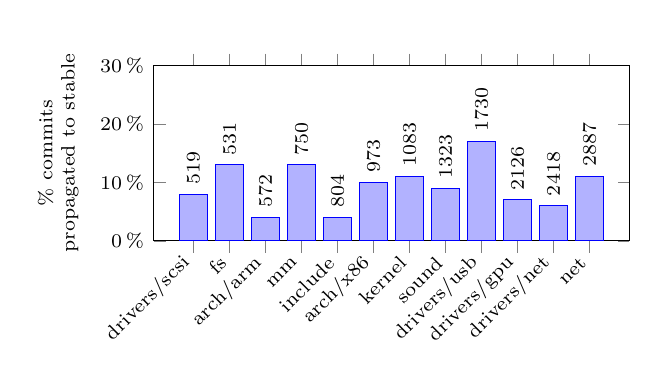
\begin{tikzpicture}
\begin{axis}[ybar,xtick=data,ticklabel style = {font=\scriptsize},
 label style = {font=\scriptsize},
 x tick label style={rotate=45,anchor=east, yshift=-0.01em},
ylabel={\begin{tabular}{c}\% commits\\propagated to stable\end{tabular}},
yticklabel=\pgfmathprintnumber{\tick}\,$\%$,
        ymin=0,
        ymax=30,
symbolic x
    coords={drivers/scsi,fs,arch/arm,mm,include,arch/x86,kernel,sound,drivers/usb,drivers/gpu,drivers/net,net}]
\addplot coordinates
{(drivers/scsi,                   8)
(fs,                             13)
(arch/arm,                       4)
(mm,                             13)
(include,                        4)
(arch/x86,                       10)
(kernel,                         11)
(sound,                          9)
(drivers/usb,                    17)
(drivers/gpu,                    7)
(drivers/net,                    6)
(net,                            11)};

\node[below,rotate=90,anchor=west] at (axis cs:drivers/scsi,8) {\scriptsize 519};
\node[below,rotate=90,anchor=west] at (axis cs:fs,13) {\scriptsize 531};
\node[below,rotate=90,anchor=west] at (axis cs:arch/arm,4) {\scriptsize 572};
\node[below,rotate=90,anchor=west] at (axis cs:mm,13) {\scriptsize 750};
\node[below,rotate=90,anchor=west] at (axis cs:include,4) {\scriptsize 804};
\node[below,rotate=90,anchor=west] at (axis cs:arch/x86,10) {\scriptsize 973};
\node[below,rotate=90,anchor=west] at (axis cs:kernel,11) {\scriptsize 1083};
\node[below,rotate=90,anchor=west] at (axis cs:sound,9) {\scriptsize 1323};
\node[below,rotate=90,anchor=west] at (axis cs:drivers/usb,17) {\scriptsize 1730};
\node[below,rotate=90,anchor=west] at (axis cs:drivers/gpu,7) {\scriptsize 2126};
\node[below,rotate=90,anchor=west] at (axis cs:drivers/net,6) {\scriptsize 2418};
\node[below,rotate=90,anchor=west] at (axis cs:net,11) {\scriptsize 2887};

\end{axis}
\end{tikzpicture}
\caption{Percentage of mainline commits propagated to stable kernels for
  the 12 directories with the most stable commits. The number above each bar
  indicates the number of propagated commits.}
\label{pctprop}
\end{figure}

Figure \ref{pctcom} shows the percentage of mainline commits propagated to
stable kernels that contain the Cc: stable tag, for the same set of kernel
directories.  The rate is very low for {\tt drivers/net} and {\tt net},
which are documented to have their own procedure \cite{stabledoc}.  The
others mostly range from 60\% to 85\%.  Commits in stable kernels that do
not contain the tag are commits that the stable maintainers have identified
on their own or that they have received via other non-standard channels.
This represents further work that can be saved by an automatic labeling
approach.

\begin{figure}
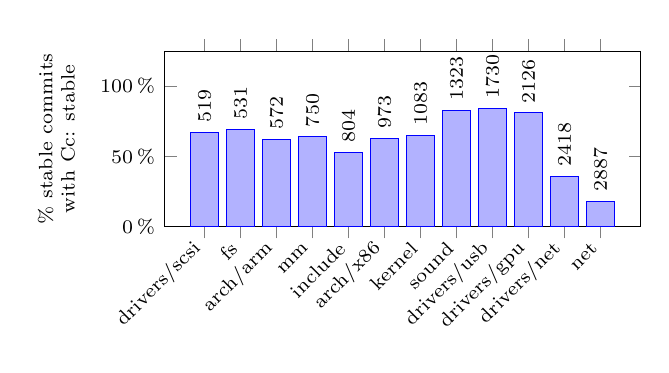
\begin{tikzpicture}
\begin{axis}[ybar,xtick=data,ticklabel style = {font=\scriptsize},
 label style = {font=\scriptsize},
 x tick label style={rotate=45,anchor=east, yshift=-0.01em},
ylabel={\begin{tabular}{c}\% stable commits\\with Cc: stable\end{tabular}},
yticklabel=\pgfmathprintnumber{\tick}\,$\%$,
        ymin=0,
        ymax=125,
symbolic x
    coords={drivers/scsi,fs,arch/arm,mm,include,arch/x86,kernel,sound,drivers/usb,drivers/gpu,drivers/net,net}]
\addplot coordinates
{(drivers/scsi,                   67)
(fs,                             69)
(arch/arm,                       62)
(mm,                             64)
(include,                        53)
(arch/x86,                       63)
(kernel,                         65)
(sound,                          83)
(drivers/usb,                    84)
(drivers/gpu,                    81)
(drivers/net,                    36)
(net,                            18)};

\node[below,rotate=90,anchor=west] at (axis cs:drivers/scsi,67) {\scriptsize 519};
\node[below,rotate=90,anchor=west] at (axis cs:fs,69) {\scriptsize 531};
\node[below,rotate=90,anchor=west] at (axis cs:arch/arm,62) {\scriptsize 572};
\node[below,rotate=90,anchor=west] at (axis cs:mm,64) {\scriptsize 750};
\node[below,rotate=90,anchor=west] at (axis cs:include,53) {\scriptsize 804};
\node[below,rotate=90,anchor=west] at (axis cs:arch/x86,63) {\scriptsize 973};
\node[below,rotate=90,anchor=west] at (axis cs:kernel,65) {\scriptsize 1083};
\node[below,rotate=90,anchor=west] at (axis cs:sound,83) {\scriptsize 1323};
\node[below,rotate=90,anchor=west] at (axis cs:drivers/usb,84) {\scriptsize 1730};
\node[below,rotate=90,anchor=west] at (axis cs:drivers/gpu,81) {\scriptsize 2126};
\node[below,rotate=90,anchor=west] at (axis cs:drivers/net,36) {\scriptsize 2418};
\node[below,rotate=90,anchor=west] at (axis cs:net,18) {\scriptsize 2887};

\end{axis}
\end{tikzpicture}
\caption{Percentage of mainline commits propagated to stable kernels that
  contain a Cc: stable tag for the 12 directories with the most mainline
  commits propagated to stable kernels. The number above each bar indicates
the number of propagated commits.}
\label{pctcom}
\end{figure}

\subsection{Challenges for Machine Learning}
\label{sec:challenges}

Stable patch identification poses some unique challenges for machine learning.
These include the kind of information available in a Linux kernel patch and the
diversity in the reasons why patches are or are not selected for application to stable
kernels.

First, Linux kernel commit logs are written free-form. While maintainers
are asked to add a ``Cc: stable@vger.kernel.org'' tag to commits that
should be propagated to stable versions, they may neglect to do this.  
% Our
% goal is to identify stable-relevant commits for which adding this tag has
% been overlooked, and thus we ignore this information \jl{Maybe this
%   sentence is not needed here; it is more about our dataset. which comes
%   later.}. 
  Patches also contain a combination of text, represented by the
commit log, and code, represented by the enumeration of the changed
lines. Code is structured differently than text, and thus we need to
construct a representation that enables machine learning algorithms to
detect relevant properties.

Second, some patches applied to stable kernels are not bug fixing
patches. The stable documentation itself stipulates that patches adding new
device identifiers are also acceptable. Such patches represent a very simple form
of new functionality, implemented as an array element initialization, but they are
allowed in stable kernels because they are unlikely to cause problems for users of
stable kernels and may enable the use of the stable kernel with new device variants.
% These patches have a common structure and are easily recognized, and thus should
% not pose a significant challenge for machine learning. 
Another reason that a non bug
fixing patch may be introduced into a stable kernel is that a subsequent bug
fixing patch depends on it. 
These non bug fixing patches, which typically perform
refactorings, should satisfy the criteria of being small and obviously correct, but
may have other properties that differ from those of bug-fixing patches. They may
thus introduce apparent inconsistencies into the machine learning process.

Finally, some patches may perform bug fixes, but may be correctly not propagated to
stable. One reason is that some parts of the code change so rapidly that the patch
does not apply cleanly to any stable version. Another reason is that the bug was
introduced since the most recent mainline release, and thus does not appear in any
stable version.

As the decision of whether to apply a patch to a stable kernel depends in part
on factors external to the patch itself, we cannot hope to achieve a perfect solution
based on applying machine learning to patches alone. 
% Still, stable-kernel maintainers
% have reported to us that they are able to check likely stable-relevant patches
% quickly (e.g., 32 in around 20 minutes).\footnote{Greg Kroah Hartman, private communication, April 28, 2017}. 
Still, we believe that we can effectively
complement existing practice by orienting stable-kernel maintainers towards
likely stable-relevant commits that they may have overlooked, even though
the above issues introduce the risk of some false negatives and false positives.


\section{Proposed Approach}
\label{sec:approach}
% \jh{Comment 1: Need to explain PatchNet in a good way so that non-expert ML can understood (reviewer A) -- Need to rewrite the section~\ref{sec:approach}}

In this section, we first formulate the problem and provide an overview of PatchNet. We then describe the details of each module inside PatchNet. Finally, we present an algorithm for learning effective settings of PatchNet's parameters.
% Finally, we present the algorithms for learning model parameters.

\vspace{-0.5em}
\subsection{Framework Overview}
\label{sec:overall_framework}

The goal of PatchNet is to automatically label a
patch as stable or non-stable in order to reduce the manual effort for the stable-kernel maintainers. 
% Let $\mathcal{X} = \{x_1, \dots, x_N \}$ denote
% the set of patches that have been accepted into the mainline kernel, where
% $N$ is the number of patches considered.
% \jl{Do we ever use $N$? If not, drop this explanation.} \jl{I put this
%   question back because I still don't see where we use $N$}.
We consider the identification of stable patches as a learning task to construct a prediction function $f:
\mathcal{X} \longmapsto \mathcal{Y}$, where $\mathcal{Y} = \{0, 1\}$. In
this case, $x_i \in \mathcal{X}$ is identified as a stable patch when $f(x_i) = 1$, and 0 otherwise.
% $y_i \in \mathcal{Y}$ 
% \jl{Why say $y_i$ instead of $f(x_i)?$}
% \jg{$y_i$ is the true label and $f(x_i)?$ is the predicted label}
% \jl{It doesn't say that anywhere at all.}
% is 1 when patch $x_i \in \mathcal{X}$ is identified as a
% stable patch, and 0 otherwise.

As illustrated in Figure~\ref{fig:patchnet}, PatchNet consists of three
main modules: (1) a \textit{commit message module}, (2) a \textit{commit
  code module}, and (3) a \textit{classification module}.  The first two
are built upon a CNN-based architecture~\cite{lecun1998gradient, krizhevsky2012imagenet}, and aim
to learn a representation of the textual commit message
(cf. Figure~\ref{fig:sample_patch}, lines 5-12) and the set of diff code
elements (cf. Figure~\ref{fig:sample_patch}, lines 14-28) of a patch,
respectively.  The \textit{commit message module} and the \textit{commit
  code module} transform the commit message and the code changes into
embedding vectors $\mathbf{e}_m$ and $\mathbf{e}_c$, respectively. The two
vectors are then passed to the \textit{classification module}, which aims to compute a prediction score indicating the likelihood of a patch being a stable patch.
% \ty{pls verify}

\begin{figure}[!t]
	\center
	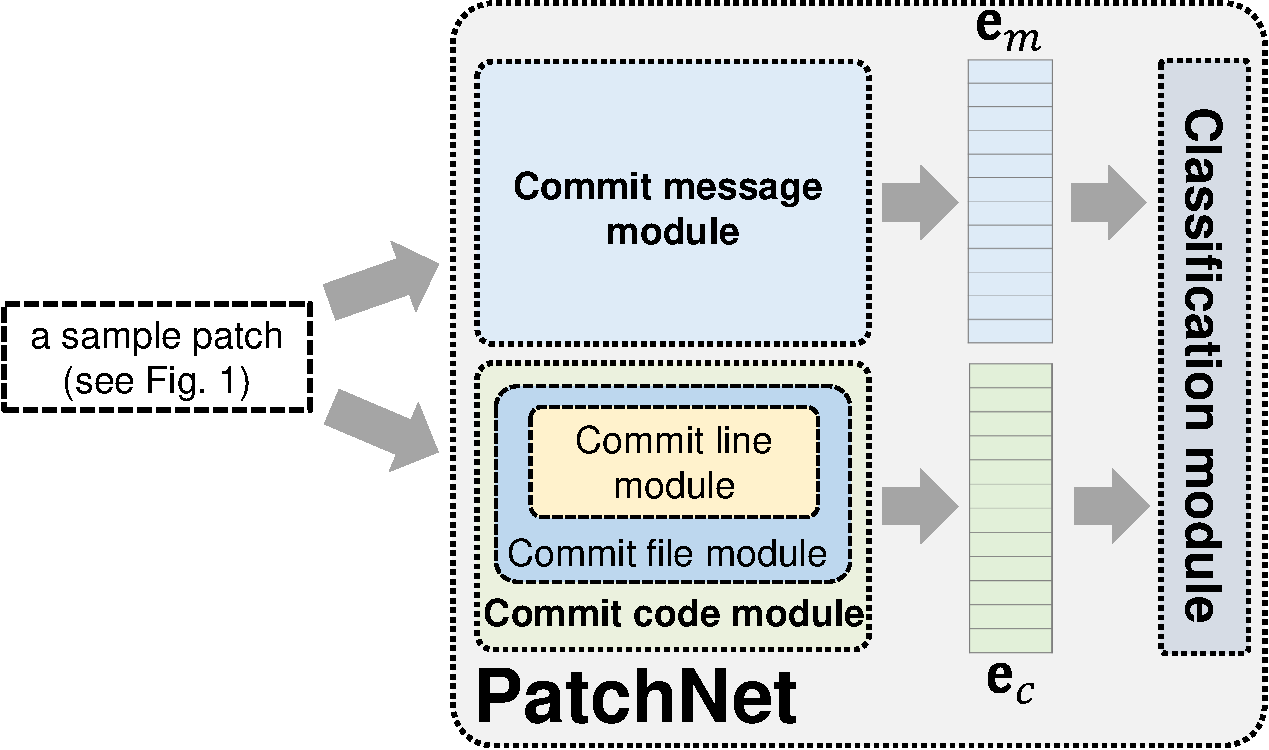
\includegraphics[scale=0.37]{figures/framework_overall_ver1.pdf}
	\caption{The proposed PatchNet framework. $\textbf{e}_m$ and $\textbf{e}_c$ are embedding vectors collected from the commit message module and commit code module respectively.}
	\label{fig:patchnet}
    \vspace{-0.4cm}
\end{figure}

\subsection{Commit Message Module}
\label{sec:commit_msg_model}

%The design of our \textit{commit message module} is built on the work of Kim~\cite{kim2014convolutional} and Kalchbrenner {\em et al.}~\cite{kalchbrenner2014convolutional} on sentence classification. 

%Figure~\ref{fig:msg_model} shows the architecture of the commit message module. The module uses CNN and involves an input message, represented as a two-dimensional matrix, a set of filters for identifying features in the message, and a means of combining the results of the filters into an \textit{embedding vector} that represents the most salient features of the message, to be used as a basis for classification.

Figure~\ref{fig:msg_model} shows the architecture
of the commit message module, which is the same as the one proposed by Kim~\cite{kim2014convolutional} for sentence classification. This module takes a commit message as input and outputs an embedding vector that represents the most salient features of the message.


\begin{figure}
\center
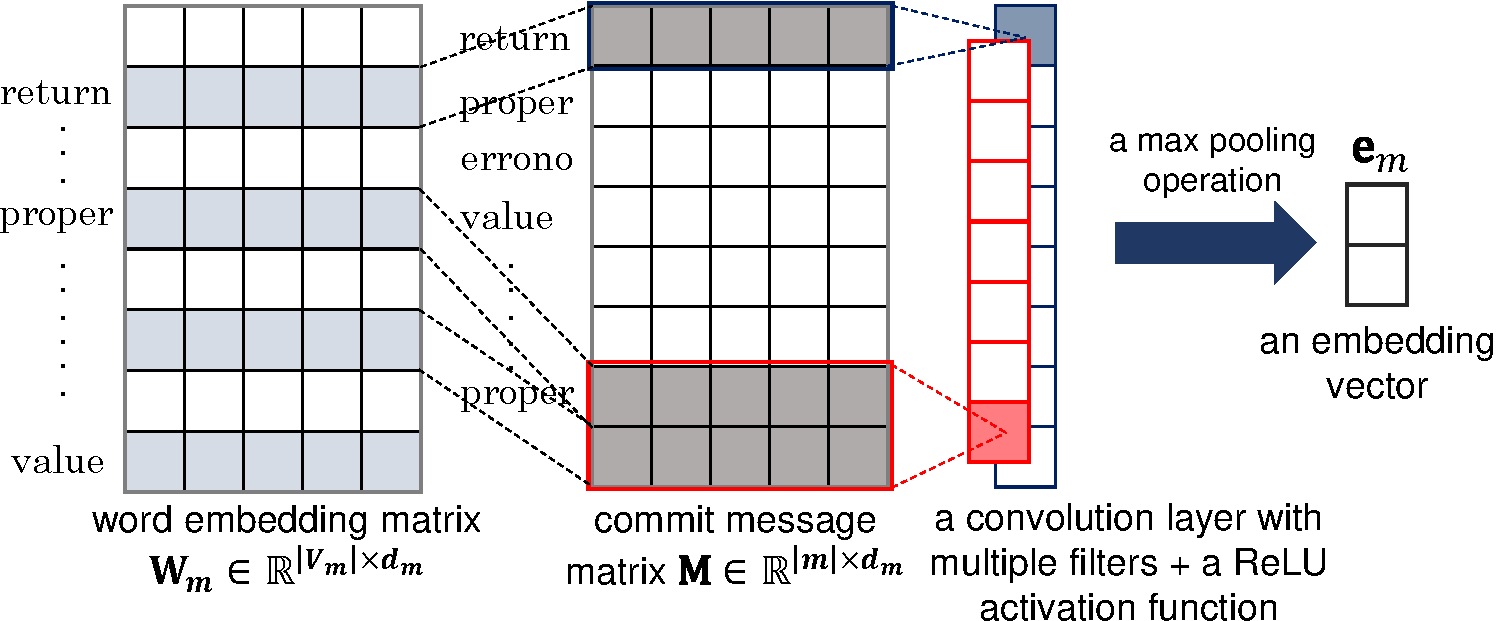
\includegraphics[scale=0.36]{figures/msg_model_ver2.pdf}
\caption{Architecture of our \textit{commit message module} used to build an embedding vector from a commit message.}
\label{fig:msg_model}
\vspace{-0.4cm}
\end{figure}

% \jl{Figure \ref{fig:msg_model} should have only two entries in the
%   embedding vector.}

\textbf{Message representation}. We encode a commit message as a
two-dimensional matrix by viewing the message as a sequence of vectors
where each vector represents one word appearing in the
message. The embedding vectors of the individual words are maintained using a
lookup table, the {\em word embedding matrix}, that is shared across all
messages.

Given a message $m$ as a sequence of words
$[\texttt{w}_1, \dots, \texttt{w}_{|m|}]$ and a word embedding matrix
$\textbf{W}_m \in \mathbb{R}^{|V_m|\times d_m}$, where $V_m$ is the vocabulary containing all words in commit messages and  $d_m$ is the
dimension the representation of a word, the matrix representation
$\textbf{M} \in \mathbb{R}^{|m| \times d_m}$ of the message is:
\begin{equation} \footnotesize
\textbf{M} =
[\textbf{W}[\texttt{w}_1], \dots, \textbf{W}[\texttt{w}_{|m|}]]
\end{equation}
For parallelization, all messages are padded or truncated to same length.

\textbf{Convolutional layer}. The role of the convolutional layer is to apply
filters to the message, in order to identify the message's salient
features.  
% \jl{convolution or convolutional?} \jg{It's the convolutional layer, more details can be found \href{https://en.wikipedia.org/wiki/Convolutional_neural_network}{here}}
%In our setting \jl{Can we drop ``In our setting''?}, 
A filter $\textbf{f} \in \mathbb{R}^{k \times d_m}$ is
a small matrix 
% \ty{actually, i feel it is product of f and M, not element-wise product...btw, f looks like a function, but it is a weight matrix, a little bit confusing here.} 
that is applied
to a window of $k$ words to produce a new feature. A feature $t_i$ is generated from a window of words
$\textbf{M}_{i:i+k-1}$ starting at word $i \leq |m|- k + 1$ by:
% \jl{$i \leq |m|- k+1$???}
\begin{equation} \footnotesize
\label{eq:filtering}
t_i = \alpha ( \textbf{f} \ast \textbf{M}_{i:i+k-1} + b_i) 
\end{equation}
where $\ast$ is a sum of element-wise products, $b_i \in
\mathbb{R}$ is a bias value, and $\alpha(\cdot)$ is a non-linear activation
function. For $\alpha(\cdot)$, we choose the rectified linear unit (ReLU) activation function~\cite{nair2010rectified}, as it has been shown to have better performance than 
its alternatives~\cite{anastassiou2011univariate,dahl2013improving}.
% logistic sigmoid and hyperbolic tangent~\cite{anastassiou2011univariate,dahl2013improving}.
%\jl{not grammatical, and I don't know what is meant}\ty{modified}
% significant benefits in terms of \jl{could we drop ``significant benefits
% in terms of''? It seems like a lot of words for no meaning.} 
%faster training, sparse activation, and
%reduced likelihood of vanishing %gradients~\cite{han1995influence,anastassiou2011univariate,dahl2013improving}. 
The filter $\textbf{f}$ is applied to all windows of size $k$ in the message resulting in a \textit{feature vector} $\textbf{t} \in \mathbb{R}^{|m|-k+1}$:
\begin{equation} \footnotesize
\label{eq:ftr_vector}
\textbf{t} = [t_1, t_2, \cdots, t_{|m|-k+1}]
\end{equation}


\textbf{Max pooling}. 
To characterize the commit message, we are interested in the degree to
which it contains various features, but not where in the message those
features occur. Accordingly, for each filter,
% To capture the most important feature in each feature vector, 
we apply a max pooling operation~\cite{collobert2011natural} over the feature vector $\textbf{t}$ to obtain the highest value:
% and take the maximum value as the feature corresponding to a particular filter:
\begin{equation} \footnotesize
\label{eq:pooling}
\underset{1 \leq i \leq |m|-k+1}{\max} t_i
\end{equation}

\noindent
The results of applying max pooling to the feature vector resulting from
applying each filter are then concatenated to form an embedding vector
($\mathbf{e}_m$ on the right side of Figure~\ref{fig:msg_model})
representing the meaning of the message.
% \jg{Look at David's comment}

\subsection{Commit Code Module}
\label{sec:commit_code_model}
Like the commit message,
the commit code can be viewed as a sequence of words. This view, however, overlooks the structure of code changes, as needed to distinguish between changes to different files, changes in
different hunks, and different kinds of changes (removals or additions). To incorporate this structural information, PatchNet contains a {\em Commit Code Module} that takes as input the code changes in a given patch and outputs an embedding vector that represents the most salient features of the code changes. The Commit Code Module contains a {\em Commit File Module} that automatically builds an embedding vector representing the code changes made to a given file in the patch. The embedding vectors of code changes at file level are then concatenated into a single vector representing all the code changes made by the patch.

\subsubsection{Commit file module}
\label{sec:code_file_framework}

The goal of the commit file module is to build an embedding vector
for each file in the patch that represents the changes that affect the file.

As shown in Figure~\ref{fig:commit_code_model}, the commit file module
takes as input two matrices (denoted by ``--'' and ``+'' in
Figure~\ref{fig:commit_code_model}) representing the removed code and added
code for the affected file in a patch, respectively. These two matrices
are passed to the \textit{removed code module} and the \textit{added code
module}, respectively, to construct corresponding embedding vectors. The two embedding vectors are then concatenated to represent the code changes in each affected file. We present the removed code module and the added code module below.

\begin{figure}[t!]
	\center
	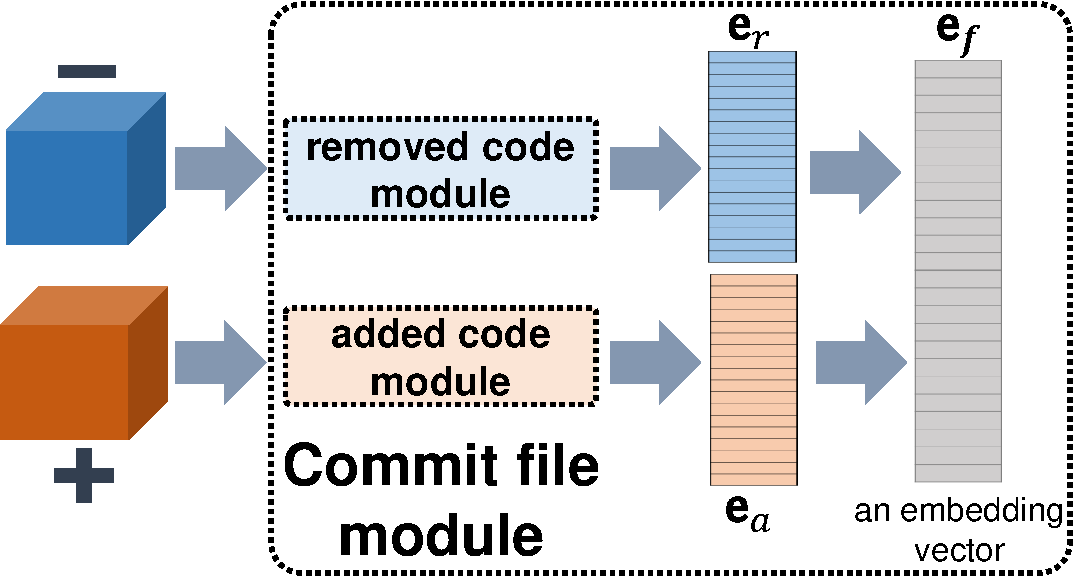
\includegraphics[scale=0.43]{figures/commit_file_model.pdf}
	\caption{Architecture of the \textit{commit file module} for
          mapping a file in a given patch to an embedding vector. The input
          of the module is the removed code and added code of the affected
          file, denoted by ``--'' and ``+'', respectively.}
	\label{fig:commit_code_model}
\end{figure}

\textbf{\textit{Removed code module.}} Figure~\ref{fig:cnn3d}
shows the structure of the \textit{removed code module}. The
input of this module is a three-dimensional matrix, indicating the removed code
in a file of a given patch, denoted by $\mathcal{B}_r \in
\mathbb{R}^{\mathcal{H} \times \mathcal{N} \times \mathcal{L}}$, where
$\mathcal{H}$, $\mathcal{N}$, and $\mathcal{L}$ are the number of hunks,
the number of removed code lines for each hunk, and the number of words of each
removed code line in the affected file, respectively. This module
constructs an embedding vector (denoted by $\textbf{e}_r$ in Figure~\ref{fig:commit_code_model}) representing the removed code in the affected file.

\begin{figure*}[t!]
	\center
	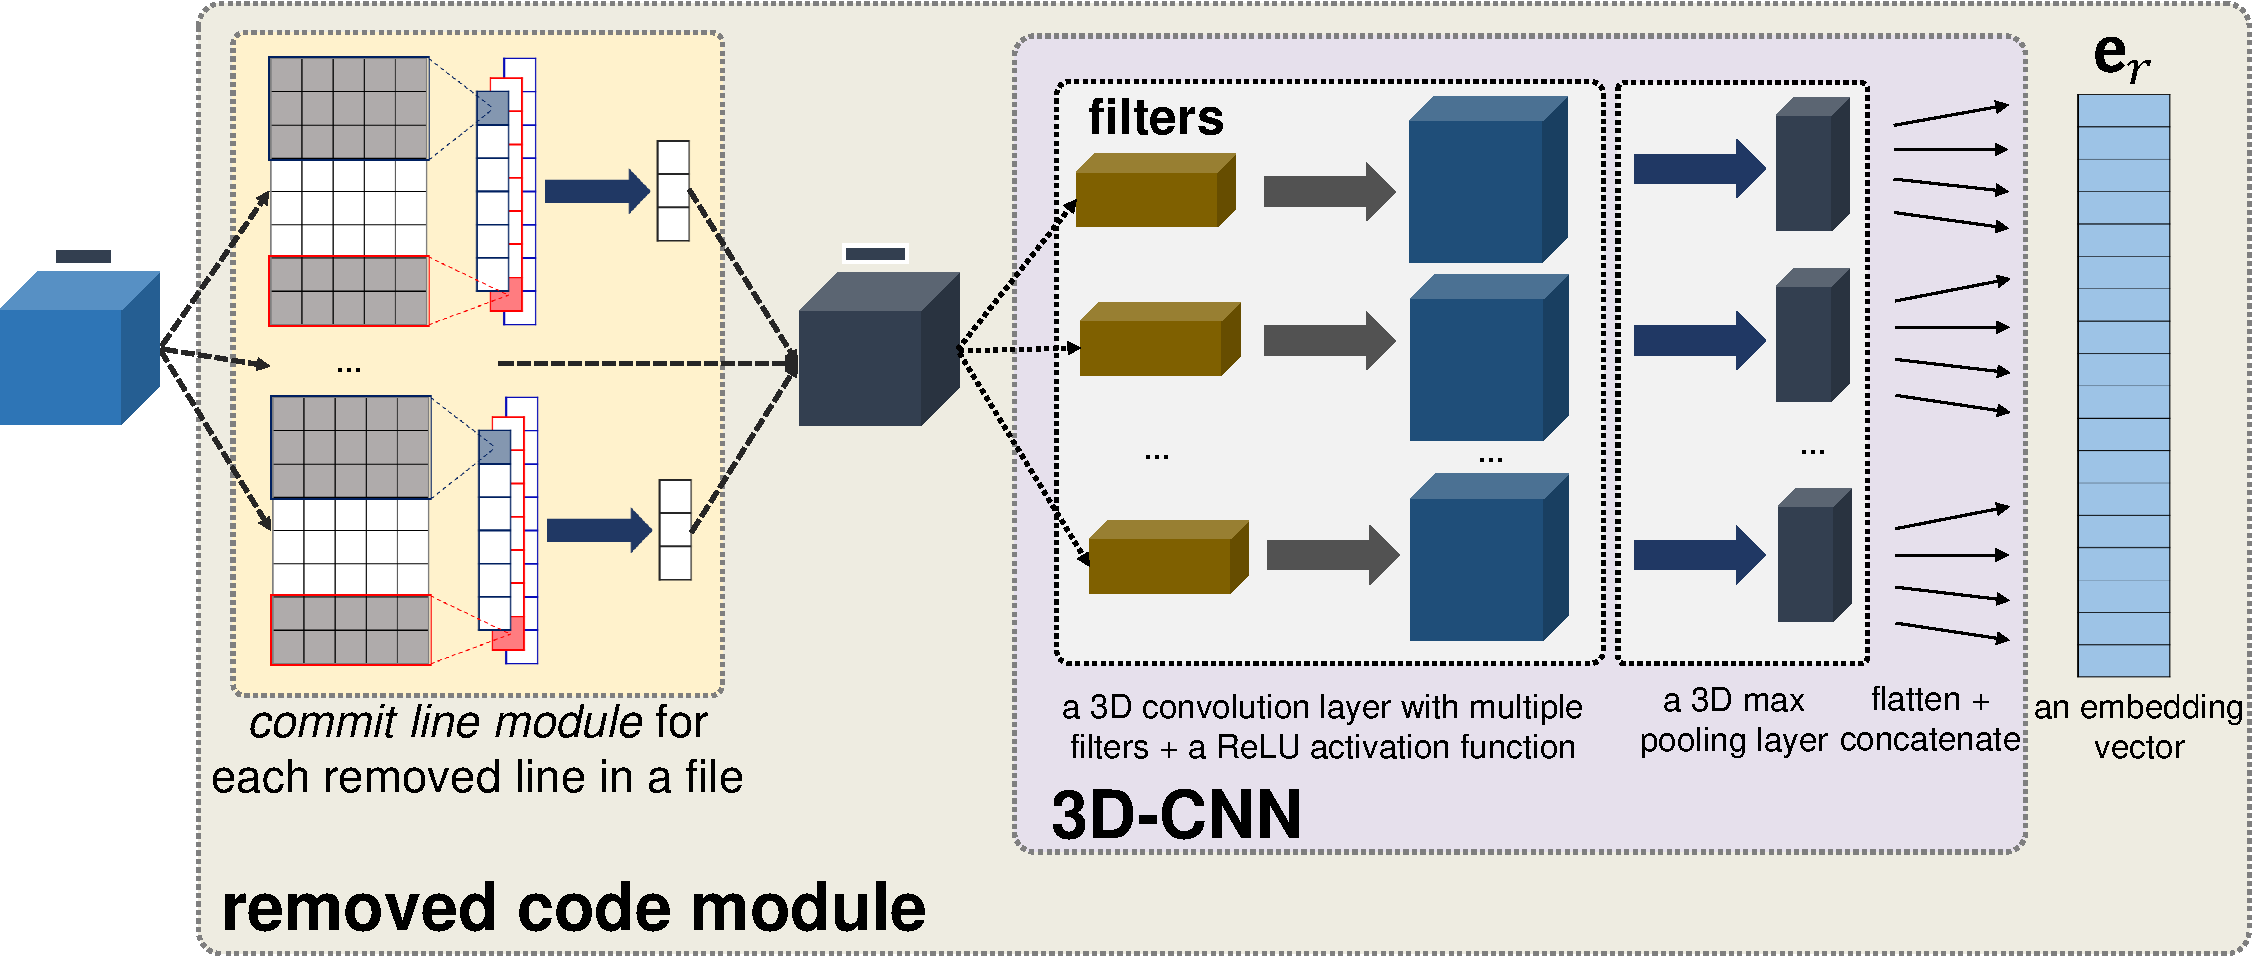
\includegraphics[scale=0.38]{figures/cnn-3d_ver1.pdf}
	\caption{Architecture of the \textit{removed code module} used to build an embedding vector for the code removed from an affected file.}
	\label{fig:cnn3d}
\end{figure*}

\textit{a) Commit line module.}  Each line of removed code in
$\mathcal{B}_r$ is processed by the {\em commit line module} to obtain a
list of embedding vectors representing the removed code lines. This module
has the same structure as the commit message module, but maintains a
code-specific vocabulary and word embedding matrix, as a word may have
different meanings in a textual message and in source code.

The obtained commit line vectors are used to construct a new three-dimensional matrix,
$\hat{\mathcal{B}}_r \in \mathbb{R}^{\mathcal{H} \times \mathcal{N} \times
  E}$. $\hat{\mathcal{B}}_r$ represents a sequence of ${\mathcal{H}}$
hunks; each hunk has a sequence of removed lines, where each line is now
represented as a $E$-dimensional embedding vector ($e_{ij} \in \mathbb{R}^E$) extracted by
the \textit{commit line module}. $\hat{\mathcal{B}}_r$ is then passed to the
3D convolutional neural network (3D-CNN), described below, to construct an embedding vector for the code removed from a file by a given patch.

\textit{b) 3D-CNN}.
% \ty{this is a module or a layer? it contains multiple layers right?} \jg{It's a filter}
The 3D convolutional layer is used to
extract features from the code removed from the affected file, as
represented by $\hat{\mathcal{B}}_r$.  This layer applies each
filter $\textbf{F} \in \mathbb{R}^{k \times \mathcal{N} \times E}$
to a window of $k$ hunks $\textbf{H}_{i:i+k-1}$ to build a new feature as
follows:
\begin{equation} \footnotesize
\label{eq:3d_filter}
f_i = \alpha(\textbf{F} \ast \textbf{H}_{i:i+k-1} + b_i) ]
\end{equation}
% \ty{make sure its element-wise or dots}
$\ast$ is the sum of element-wise products, $\textbf{H}_{i:i+k-1} \in
\mathbb{R}^{|i:i+k-1| \times\mathcal{N} \times E}$ is constructed from the
$i$-th hunk through the $(i+k-1)$-th hunk in the removed code of the affected
file, $b_i \in \mathbb{R}$ is the bias value, and $\alpha(\cdot)$ is the
ReLU activation function. As in Section~\ref{sec:commit_msg_model}, we
choose $k \in \{1, 2\}$. 
% Figure~\ref{fig:filtering_example} shows an example of a 3D convolutional layer that has one filter.
%\begin{figure}[t!]
%	\center
%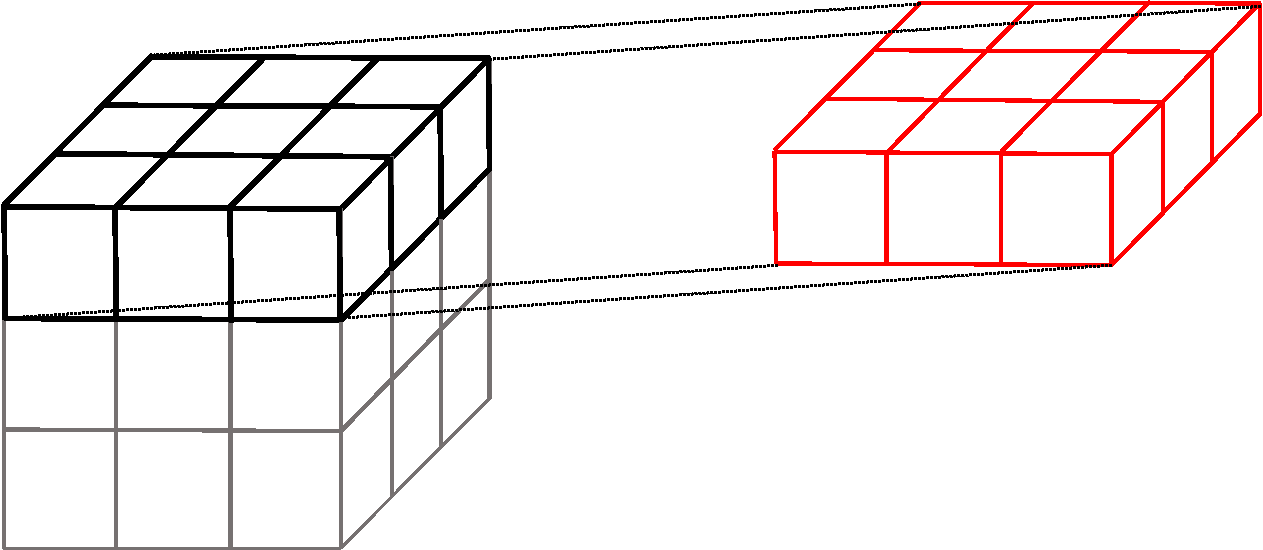
\includegraphics[scale=0.25]{figures/filtering_example.pdf}
%	\caption{A 3D convolutional layer on $3 \times 3 \times 3$ data. The $1 \times 3 \times 3$ red cube on the right is the filter. The dotted lines indicate the sum of element-wise products over all three dimensions. The result is a scalar in every instance of the operation.}
%	\label{fig:filtering_example}
%    \vspace{-0.4cm}
%\end{figure}
Applying the filter $\textbf{F}$ to all windows of hunks in
$\hat{\mathcal{B}_r}$ produces a feature vector: 
\begin{equation} \footnotesize
\label{eq:ftr_hunk}
\mathcal{F} = [f_1, \dots, f_{\mathcal{H} - k + 1}]
\end{equation}

As in Section~\ref{sec:commit_msg_model}, we apply a max pooling operation
to $\mathcal{F}$ to obtain the most important feature.
% , {\em i.e.}, the most important hunks representing information about the removed code changes. 
The features selected by max pooling with multiple filters are concatenated to
construct an embedding vector $\textbf{e}_r$ representing information
extracted from the removed code changes in the affected file.
%of a given patch. 
%(see the last layer in Figure~\ref{fig:cnn3d}).

\textbf{\textit{Added code module}} The \textit{added code module} follows
the same architecture as the removed code module. These changes in the
added and removed code are furthermore padded or truncated to have the same
number of hunks ($\mathcal{H}$), number of lines for each hunk
($\mathcal{N}$), and the number of words of each line ($\mathcal{L}$) for
parallelization. Moreover, both modules also share the same vocabulary and
use the same word embedding matrix.

The added code module
constructs an embedding vector (denoted by $\textbf{e}_a$ in Figure~\ref{fig:commit_code_model}) representing the added code in a file
of a given patch. An embedding vector representing all of the changes made to a given file by a commit is constructed by
concatenating the two embedding vectors representing the removed code and
added code, i.e., $\textbf{e}_\texttt{f} = \textbf{e}_r \oplus \textbf{e}_a$. 

% \jg{Julia: can you please recheck these two paragraph above?}

%\begin{equation} \footnotesize
%\label{eq:commit_file}
%\textbf{e}_\texttt{f} = \textbf{e}_r \oplus \textbf{e}_a
%\end{equation}  

% For parallelization, the removed and added code are furthermore padded or truncated to be the same number of hunks, number of lines for each hunk, and number of words per line.

\subsubsection{Constructing an embedding vector for commit code}
\label{sec:construct_commit_code}
The embedding vector for all the changes performed by a given patch is constructed as follows:
\begin{equation} \footnotesize
\label{eq:commit_code_vector}
\textbf{e}_c = \textbf{e}_{\texttt{f}_1} \oplus \dots \oplus \textbf{e}_{\texttt{f}_v}
\end{equation}
where $\oplus$ is the concatenation operator, $\texttt{f}_i$ denotes the $i$-th file affected by the given commit, $v$ is the number of affected files, and $\textbf{e}_{\texttt{f}_i}$ denotes the vector constructed by applying the commit file module to the affected file $\texttt{f}_i$.


\subsection{Classification Module}
\label{sec:classification_model}

\begin{figure}[t!]
	\center
	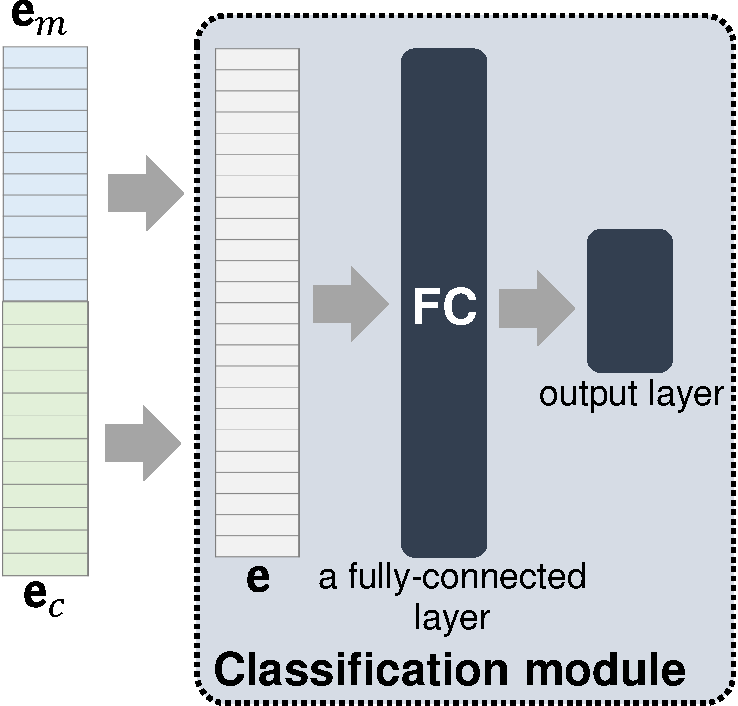
\includegraphics[scale=0.4]{figures/classification_module.pdf}
	\caption{Architecture of the \textit{classification module}, comprising a fully connected layer (FC), and an output layer.}
	\label{fig:clf_module}
    \vspace{-0.4cm}
\end{figure}

% \jl{Figure \ref{fig:clf_module} mentions a concatenation operator, but we
%   don't see it}

Figure~\ref{fig:clf_module} shows the architecture of the \textit{classification module}. It takes as input the commit message embedding vector $\mathbf{e}_m$ and the commit code embedding vector $\mathbf{e}_c$ discussed in Sections~\ref{sec:commit_msg_model} and~\ref{sec:commit_code_model}, respectively.
These two vectors are then concatenated to form a single vector representing a patch,
{\em i.e.}, $\textbf{e} = \mathbf{e}_m \oplus \mathbf{e}_c$.

We then feed the concatenated vector $\mathbf{e}$ into a fully-connected
(FC) layer, which outputs a vector
% representation \jl{what is it?} 
$\mathbf{h}$ as follows:
\begin{equation}  \footnotesize
\label{eq:fully_layer}
\mathbf{h} = \alpha(\mathbf{w}_h \cdot \mathbf{e} + b_h)
\end{equation}
where $\cdot$ is a dot product, 
% $\textbf{w}_h$ is the weight vector of the FC layer, 
$\textbf{w}_h$ is a weight matrix of the vector $\mathbf{e}$ and the FC layer and is learned during a training process,  
$b_h$ is the bias value, and $\alpha(\cdot)$ is a non-linear
activation function. Again, we use ReLU to realize $\alpha(\cdot)$.

Finally, the vector $\mathbf{h}$ is passed to an output layer, which
computes a probability score for a given patch:
\begin{equation}  \footnotesize
z_i = p(y_i=1|x_i) = \frac{1}{1 + \exp({-\mathbf{h} \cdot \mathbf{w}_o)}}
\end{equation}
% where $\mathbf{w}_o$ is the 
% weight vector of the output layer.
where $\mathbf{w}_o$ is a weight matrix 
% between the FC layer and the output layer, $\mathbf{w}_o$ 
that is also learned during our training process. 

% \jl{There is $\mathbf{\theta}$ here and $\mathbf{\theta}$ in the next
%   section, but I have no idea whether they are representing the same things.} \jg{No, they don't.}

\subsection{Parameter Learning}
\label{sec:learning}

During the training process, PatchNet learns the following parameters: the
word embedding matrices for commit messages and commit code, the filter matrices and bias of the convolutional layers, and the weights and bias of
the fully connected layer and the output layer. Training minimizes the
following standard regularized loss function~\cite{haykin2001kalman}:
\begin{equation} \footnotesize
\label{eq:cost}
\begin{split}
\mathcal{O} &= -\log\left( \prod_{i=1}^{N} p(y_i|x_i) \right) + \frac{\lambda}{2} \|\theta\|_{2}^{2} \\
 &= -\sum_{i=1}^{N} \left[ y_i \log (z_i) + (1 - y_i) \log(1 - z_i) \right] + \frac{\lambda}{2} \|\theta\|_{2}^{2}
\end{split}
\end{equation}
where $z_i$ is the probability score from the output layer and $\theta$
contains all parameters our model. 
% optimized by the network:
% \begin{align*}
% \label{eq:parameters}
% \theta = \{\textbf{W}_m, \textbf{f}, \textbf{b}, \textbf{w}_h, \text{w}_o \}
% \end{align*}
% namely the word embeddings matrix 

The term $\frac{\lambda}{2} \|\theta\|_{2}^{2}$ is used to mitigate data overfitting by penalizing large model parameters, thus reducing the model complexity. 
%Data overfitting is a common issue for neural networks, especially when the data size is small~\cite{caruana2001overfitting}. 
%To mitigate data ovefitting, 
To further improve the robustness of our model, we also apply the dropout technique~\cite{srivastava2014dropout} on the convolutional and fully-connected layers in PatchNet. 
% we add an $l_2$ regularization term \jl{It is not clear what this is.  A
%   term like the one shown here seems to be already in the above formula.
%   So it is not clear if you are describing that or how you further modify that.}
% ($\frac{\lambda}{2} \|\theta\|_{2}^{2}$) to the loss function, which
% penalizes large model parameters, thus reducing the model complexity. 

%Dropout can be viewed as a regularization technique to prevent complex co-adaptation on training data by randomly dropping neurons (units) when training a neural network. It also constitutes an efficient way for model averaging in neural networks.

To minimize the regularized loss function in (\ref{eq:cost}), we employ a
variant of stochastic gradient descent (SGD)~\cite{bottou2010large}
called \textit{adaptive moment estimation}
(Adam)~\cite{kingma2014adam}. We choose Adam over SGD due to its computational efficiency and low memory requirements~\cite{kingma2014adam, anthimopoulos2016lung, arora2018optimization}.  
% because it has been shown to converge faster and it is less sensitive to hyperparameters~\cite{}.\ty{pls add a reference here.} 
%Adam improves the convergence speed of the conventional SGD by imposing adaptive learning rate for each parameter that is computed by keeping track of the exponentially decaying average of the past gradients. We choose Adam due to its computational efficiency and low memory requirements~\cite{kingma2014adam}.  Meanwhile, to efficiently compute the gradients in linear time (with respect to the neural network size), we use backpropagation~\cite{hagan1994training}, which is a simple implementation of the chain rule of partial derivatives.


\section{Experiments}
\label{sec:exp}

In this section, we first describe our dataset and how we preprocess it. We
then introduce all baselines and evaluation metrics. Finally, we present
our research questions and results.

\subsection{Data Collection}
\label{sec:data}

We take our data from the patches that have been committed to mainline
Linux
kernel\footnote{git://git.kernel.org/pub/scm/linux/kernel/git/torvalds/linux.git}
v3.0, released in July 2011, through v4.12, released in July 2017.  We
additionally collect information from the stable
kernels\footnote{git://git.kernel.org/pub/scm/linux/kernel/git/stable/linux.git}
that had been released as of October 2017 building on Linux kernels v3.0
through v4.13.  We consider mainline commits that are duplicated in at
least one stable version to be stable-relevant.  We also consider mainline
commits to so-called ``release candidates'', that are predecessors to a
mainline kernel release, to be stable-relevant when such commits are to a
release candidate that is after the first one for a given version.  Indeed,
commits to these release candidates are expected to contain only bug fixes
and they can be viewed as the stable
versions of the new features proposed in the first release
candidate.  We refer to patches that are propagated to stable kernels or
are found in later release candidates as {\em stable patches} and patches
that are not propagated to stable kernels or found in later release
candidates as {\em non stable patches}.  To avoid biasing the learning
process towards either stable or non stable patches, we construct our
datasets such that the number of patches in each category is roughly
balanced.  While this situation does not reflect the number of stable and
non stable patches that confront a stable kernel maintainer each day, it
allows effective training and interpretation of the experimental results.

\subsubsection{Identifying Stable Patches}
\label{sec:stable_patch}

The main challenge in constructing the datasets is to determine which
mainline patches have been propagated to stable kernels.  Indeed, there is
no required link information connecting the two.  Some stable patches
explicitly mention the corresponding mainline commit in the commit message,
which we refer to as a {\em back link}. For others, we rely on the author
name and the subject line. Subject lines typically contain information
about both the change made and the name of the file or directory in which
the change is made, and thus should be unique.  Accordingly, we first
collect from the patches in the stable kernels a list of any back
links and a list of pairs of author name and subject line.  A commit from
the mainline whose commit id is mentioned in a back link or whose author
name and subject line are the same as one found in a patch to a stable
kernel is considered to be a stable-relevant patch.

\subsubsection{Collecting the dataset}
\label{sec:mainline_patch}

We collect our dataset from the mainline kernel.  In order to focus on
patches that are challenging for stable maintainers to classify, we drop in
advance all patches that do not meet the stable-kernel size
guidelines,\footnote{https://www.kernel.org/doc/html/v4.15/process/stable-kernel-rules.html}
{\em i.e.}, those that exceed 100 code lines, including both changed lines
and its context as reported by the {\tt diff} command.  We then keep all
identified stable patches for our dataset and select an equal number of non
stable patches.  When possible, we select non stable patches that have a
similar number of changed lines as the stable patches, again to create a
dataset that reflects the cases that cannot be excluded by size alone and
thus are challenging for stable kernel maintainers.  These patches are then
subject to a preprocessing step that is detailed in the next section.

Our dataset comes from Linux kernel mainline versions 3.0 (July 2011)
through 4.12 (July 2017). There were 424,380 commits during that period.  We
consider only those commits that are not merge commits, that modify a file
as opposed to only adding or removing files, and that affect at least one
{\tt .c} or {\tt .h} file.  This leaves 346,570 commits (82\%).  Of these
346,570 commits, 79,319 (23\%) are not considered because they contain more
than 100 changed lines, leaving 267,251 commits.  Of these, we pick the
42,408 stable patches for which the preprocessing step is successful and
39,995 non-stable patches, {\em i.e.}, 82,403 patches in all.

%82597 (training) + 122,364 = 204,961 commits.  The 82,597 commits include
%all commits that have been applied to stable trees and that are in "rc"
%(release candidate) versions between rc1 and the subsequent version.  The
%commits up to rc1 are primarily adding new features, whereas the commits
%in the subsequent release candidates should increasingly consist of only
%bug fixes on the recently added features.

%In general, our training set is noisy.  Most of our stables should be bug
%fixes, but a small percentage of stables may be there for other reasons,
%such as that a bug fix depends on them or that they add a new device
%identifier that is considered to be trivial and useful enough to be worth
%making a modification to a stable version.  The whole point of our work is
%that there may be stable relevant patches the maintainers are not
%currently marking as stable and that are thus getting overlooked.  If we
%can run the algorithm on the larger dataset, then we can evaluate whether
%our approach compensates for the laziness of maintainers, by highlighting
%more patches of maintainers who are currently underreporting. But
%currently, we have no way to show that we do better than current practice.

\subsection{Patch Preprocessing}
\label{sec:patch_processing}

Our approach applies some preprocessing steps to the patches before they are
given to PatchNet.

\subsubsection{Preprocessing of commit messages}

Our approach applies various standard natural language techniques to the
commit messages, such as stop word elimination and
stemming~\cite{vijayarani2015preprocessing, brants2003natural}, to reduce
message length and eliminate irrelevant information.  Subsequently, we pad
or truncate all commit messages to the same size, specifically 512 words,
covering the complete commit message for all but two patches, for
parallelism.  Because we are interested in cases that are challenging for
the stable kernel maintainer, we drop tags such as Cc: stable and Fixes,
whose goal is to indicate that a given patch is a stable-relevant or a bug
fixing patch.  We also drop tags indicating who has approved the patch, as
the set of developers and their work profiles can change in the future.

\subsubsection{Preprocessing of code changes}
\label{sec:extract_level_diff}

Diff code elements, as illustrated in Figure~\ref{fig:sample_patch}, may
have many shapes and sizes - from a single word to multiple lines spread
out over multiple hunks. To describe changes in terms of meaningful
syntactic units and to provide context for very small changes, we collect
differences at roughly the granularity of atomic statements. These may be,
{\em e.g.}, simple assignment statements, return statements, if headers,
etc.  For example, in the patch illustrated in
Figure~\ref{fig:sample_patch}, the only change is to replace {\tt 1} on
line 22 by {\tt err} on line 23.  Nevertheless, we represent the change as
a change in the complete return statement, {\em i.e.}, {\tt return 1;} is
transformed into {\tt return err;}.  We also distinguish changes in error
checking code (code to detect whether an error has occurred, {\em e.g.}, line
21 in Figure~\ref{fig:sample_patch}) and in error handling code (code to
clean up after an error has occurred, {\em e.g.}, lines 22 and 23 in
Figure~\ref{fig:sample_patch}) from changes in other code, which we refer
to as {\em normal code}. Error checking code and error handling code are
indeed very common in the Linux kernel, which must be robust, and they are
disjoint in structure and purpose from the implementation of the main
functionality.

For a given commit, the first step is to extract the names of the affected
files and to extract the state of those files before and after the
commit. Analogous to the stemming and stop word elimination performed at
the commit message level, for each before and after file instance, we
remove comments and the contents of strings, as changes in comments and
within strings are not likely to be stable-relevant. For a given pair of
before and after files, we then compute the difference using the command
``git diff -U0 old new'', giving the changed lines with no lines of
% * <hvdthong@gmail.com> 2018-08-25T10:47:15.001Z:
%
% ^.
% * <hvdthong@gmail.com> 2018-08-25T10:47:13.368Z:
%
% ^.
surrounding context. For each ``--'' or ``+'' line in the diff output, we
then collect a record indicating the sign (``--'' or ``+''), the category
(error-handling code, etc.), the hunk number, the line number in the old or
new version, respectively, and the starting and ending columns of the
non-space changes on the line.  We furthermore keep the names of called
functions, when these are not defined in the same file and are used at
least 5 times, but drop other identifiers, {\em i.e.} field names and
variable names, as these may be too diverse to allow effective learning and unnecessarily slow down the training time.
Indeed, adding just the frequently used function names increases the code
vocabulary size from 43 to 3,616 unique tokens, which
increases the training time.

To extract changes at the level of atomic statements, rather than the
individual lines obtained by diff, we parse each file as it exists before
and after the change and keep the atomic statements that intersect with
a changed line observed by diff.  For this, we use the parser of the C
program transformation system Coccinelle~\cite{padioleau2008documenting},
which uses heuristics to parse around compiler directives and macros
\cite{yoann:cc}.  This makes it possible to reason about patches in terms
of the way they appear to the user, without macro expansion, but comes with
some cost, as some patches must be discarded because the parsing heuristics
are not sufficient to parse all of the code affected by the changed
lines. %\jl{Perhaps some numbers should appear here}

By following the above-mentioned steps, we collect the affected files of a
given patch. For each removed or added code line of the affected file,
denoted by ``--'' and ``+'', we collect a hunk number and a line number
corresponding to the removed or added code line. Each word in a line is a
pair of the associated token and the annotation indicating whether the word
occurs on a line of as error-checking code, error-handling code, or normal
code.  This information is used to build the two three-dimensional matrices
representing the removed code and the added code for the affected file
({\em cf.} Figure \ref{fig:commit_code_model}).

\subsection{Baselines}
\label{sec:baselines}
We compare PatchNet with several baselines:

\begin{itemize}[leftmargin=0.4cm]
\item Keyword: As a simple but frequently used
  heuristic~\cite{tian2012identifying}, we select all commits in which the
  commit message includes ``bug'', ``fix'', or ``bug-fix'' after conversion
  of all words to lowercase and stemming.  While not all bug fixes are
  relevant for stable kernels, as some bugs may have very low impact or the
  fix may be too large or complicated to be considered clearly correct, the
  problem of identifying bug fixes is close enough to that of recognizing
  stable relevant patches to make comparison with our model valuable.
\item LPU+SVM: This method for identifying bug-fixing patches was proposed
  by Tian et
  al.~\cite{tian2012identifying} and comprises two algorithms, i.e.,
  Learning from Positive and Unlabeled Examples
  (LPU)~\cite{joachims1999svmlight, letouzey2000learning, liu2003building}
  and Support Vector Machine (SVM)~\cite{cauwenberghs2001incremental,
    cristianini2000introduction}, which are used to build a classification
  model for automatically identifying bug fixing patches. The set of code
  features considered was manually selected. In Tian et al.'s work, stable kernels were
  considered as a source of bug-fixing patches in the training and testing
  data.

 \item LS-CNN: Huo et al.~\cite{huo2017enhancing} combined
   LSTM~\cite{hochreiter1997long} and CNN~\cite{lecun1998gradient} 
%    \jl{Could LSTM be mentioned first, since the name of the approach is
%      LS-CNN?} \jg{I'll fix it then} 
     to localize potential buggy source files based on bug report
   information. They used CNN to learn a representation of the bug report
   and a combination of LSTM and CNN 
%    \jl{again, could LSTM be mentioned
%      first?} 
     to learn the structure of the code.  To assess the ability of
   LS-CNN to classify patches as stable relevant, for a given patch, we
   give the commit message as input to LS-CNN in place of the bug
   report and the result of concatenating the lines changed in the various
   files and hunks as input to LS-CNN in place of the potential buggy
   source file.
  
% \jh{Comment 7: Missing vital references and related work discussions to justify novelty of PatchNet compared to other baselines (i.e., LSTM-CNN or LPU-SVM). Why should we choose CNN over LSTM or RNN? (reviewer B, meta reviewer)}

% \jg{Julia: I already rewrote the paragraph LS-CNN, can you please check it
%   out again?}
% \jl{I rewrote the above paragraph}

\item Feed-Forward Fully Connected Neural Network (F-NN): Inspired by the
  above-cited work of Tian et al.\ on LPU+SVM, a Linux stable kernel
  maintainer, Sasha Levin, has developed an approach to identifying
  stable patches \cite{sasha} based on a Feed-Forward Fully
  Connected Neural Network~\cite{bishop1995neural, goodfellow2016deep} and
  a set of manually selected features, including frequent commit message
  words, author names, and some code metrics.  Levin actively uses this
  approach in his work on the Linux kernel.
\end{itemize}

For LPU-SVM and LS-CNN, we used the same parameters and settings as
described in the respective papers. For F-NN, we asked Levin to train the tool on our training data and
test it with our testing data. We use 50\% as the cut off for considering a patch to be stable relevant for PatchNet and all baselines.

\subsection{Training and hyperparameters}
\label{sec:parameters}

%We empirically run PatchNet on different the number of convolutional filters and number of convolutional filter length and select the best number of convolutional filters and filter length for our model. %(i.e., $k=1$ and $k=2$) having length 64 on both \textit{commit message module} and \textit{commit code module} for training PatchNet. 

% PatchNet also has a number of other hyperparameters. 
% We set the size of PatchNet's hidden layer ($\textbf{h}$), $l_2$ regularization, and the dropout rate to be 100, $1e-5$, and 0.5, respectively. The dimensions of
% the word vectors in commit message $d_m$ and code changes $d_c$ are set to
% 50. PatchNet is trained using SGD~\cite{bottou2010large} with shuffled
% mini-batches. The batch size is set to 32. We train PatchNet for 25 epochs
% and apply the early stopping strategy~\cite{prechelt1998automatic}, i.e.,
% we stop the training if there has been no update to the loss value (see Equation~\ref{eq:cost}) for the last 5 epochs. These parameters follow a prior work~\cite{severyn2015learning}. 

% The parameters \jl{hyperparameters?} of PatchNet were chosen as follows:
% the number of convolutional filters, the size of PatchNet's hidden layer
% ($\textbf{h}$), $l_2$ regularization \jl{I don't understand what is the
%   parameter here}, and the dropout rate to be 64, 100, $1e-5$, and 0.5,
% respectively \jl{This is hard to read - the respectively is too complex.
%   Just give the numbers one by one.  Or consider making a table.}. The
% dimensions of the word vectors in commit message $d_m$ and code changes
% $d_c$ are set to 50. PatchNet is trained using SGD~\cite{bottou2010large}
% \jl{I thought we use Adam, which is different than SGD.} with shuffled
% mini-batches. The batch size is set to 32. We train PatchNet for 25 epochs
% and apply the early stopping strategy~\cite{prechelt1998automatic}, i.e.,
% we stop the training if there has been no update to the loss value (see
% Equation~\ref{eq:cost}) for the last 5 epochs. All these parameters of our
% model are in line with a prior work~\cite{severyn2015learning, yu2014deep}.

% \jh{Comment 8: Hyper-parameters: how do we select parameters for deep learning models? (reviewer C, meta reviewer)}

% \jg{Julia: can you please check this section?}

For the sizes of the filters described in Section~\ref{sec:approach}, we choose $k \in \{1, 2\}$, making the associated
windows analogous to a 1-gram or 2-gram as used in natural language
processing~\cite{jurafsky2014speech, brown1992class}. 
% \ty{I move this
%   paragraph from the approach section to here because it is a
%   parameter. Please add it to the above parameter list.} 
  Using 2-grams
allows our approach to take into account the temporal ordering of words,
going beyond the bag of words used by Tian et
al.~\cite{tian2012identifying}. The number of convolutional filters is set
to 64. The size of the fully-connected layer described in Section~\ref{sec:classification_model} is set to 100. The
dimensions of the word vectors in commit message $d_m$ and code changes
$d_c$ are set to 50. PatchNet is trained using Adam~\cite{kingma2014adam}
% \jl{I thought we use Adam, which is different than SGD.} 
with shuffled
mini-batches. The batch size is set to 32. We train PatchNet for 25 epochs
and apply the early stopping strategy~\cite{prechelt1998automatic, caruana2001overfitting}, i.e.,
we stop the training if there has been no update to the loss value (see
Equation~\ref{eq:cost}) for the last 5 epochs. All these hyperparameter values
% parameters
% \jl{hyperparameter values?}
are widely used in the deep learning community~\cite{severyn2015learning, huo2016learning, huo2017enhancing, hinton2012improving}. 
% in line with a prior work~\cite{severyn2015learning}.  

%Note that the word embedding matrices are learned during the training process. 

% ~\cite{mou2016convolutional}. 

\subsection{Evaluation Metrics}
\label{sec:metrics}
To evaluate the effectiveness of a stable patch identification
model, we employ the following metrics:

\begin{itemize}[leftmargin=0.4cm]
\item Accuracy: Proportion of stable and non-stable patches that are correctly classified.
\item Precision: Proportion of patches that are correctly classified as stable. 
\item Recall: Proportion of stable patches that are correctly classified. 
\item F1: Harmonic mean between precision and recall
\item AUC: Area under the Receiver Operating Characteristic curve. It measures if the stable patches tend to have higher predicted probabilities (to be stable) than non stable ones. 
\end{itemize}

% decision tree (DTree)~\cite{safavian1991survey}, long short-term memory (LSTM)~\cite{hochreiter1997long}, birectional long short-term memory (Bi-LSTM)~\cite{graves2005bidirectional}, convolutional neural network (CNN)~\cite{kim2014convolutional}, 

\subsection{Research Questions and Results}
\label{sec:rq}
Our study seeks to answer three research questions: 

\vspace{0.1cm}\noindent{\bf RQ1: How to decompose the dataset into training
  and testing data?}  A common strategy for evaluating machine learning
algorithms is $n$-fold cross-validation~\cite{kohavi1995study},
in which a dataset is randomly distributed among $n$ equal-sized buckets,
each of
which is considered as test data for a model trained on the contents of the
remaining $n-1$ buckets.  When data elements become available over time, as
is the case of Linux kernel patches, this strategy can result in testing a
model on data that predates some of the data on which the model was
trained.  Respecting the order in which patches are submitted,
however, would limit the amount of testing that can be done, given
the fairly small number of stable patches available.

To address this issue, we first assess whether training on future data
helps or harms the accuracy of PatchNet on our dataset.  We first sort the
patches collected in Section~\ref{sec:data} from earliest to latest based
on the date when the patch author submitted the patch to maintainers. Then,
we divide the dataset into 5 mutually exclusive sets by date. Note that the
resulting five sets are not perfectly balanced, but they come close, with
stable patches making up 45\% to 55\% of each set.  Then, we repeat the
following process five times: take one set as a testing set and use the
remaining four sets for training. When we test on the first set, we observe
the impact of training only on future data.  When we test on the fifth set,
we observe the impact of training only on past data.  The other testing
sets use models trained on a mixture of past and future data.

Table~\ref{tab:cross_valid_patchnet} shows the results of PatchNet on the
different test sets. The standard deviations are quite small (i.e., below
0.013), hence there is no difference between training on past or future
data.  Our dataset starts with Linux v3.0, which was released in 2011,
twenty years after the start of work on the Linux kernel.  The lack of
impact due to training on past or future data suggests that in such a
mature code base the properties that make a patch relevant for stable
kernels are fairly constant over time.  This property is indeed beneficial,
because it means that our approach can be used to identify stable-relevant commits that have been missed in older versions.  In subsequent research
questions, we thus retain the same five test and training sets.

\begin{table}[t!]
  \centering
  \caption{The results of PatchNet on the five chronological
    test sets}
    \begin{tabular}{|l|c|c|c|c|c|}
    \hline
          & \textbf{Accuracy} & \textbf{Precision} & \textbf{Recall} & \textbf{F1}    & \textbf{AUC} \\
    \hline
    \hline
    Set=1 & 0.852 & 0.841 & 0.886 & 0.863 & 0.850 \\
    \hline
    Set=2 & 0.860  & 0.833 & 0.909 & 0.869 & 0.859 \\
    \hline
    Set=3 & 0.866 & 0.833 & 0.910  & 0.870  & 0.867 \\
    \hline
    Set=4 & 0.864 & 0.828 & 0.912 & 0.868 & 0.864 \\
    \hline
    Set=5 & 0.869 & 0.860  & 0.917 & 0.887 & 0.862 \\
    \hline
%     \textbf{Average} & \textbf{0.862} & \textbf{0.839} & \textbf{0.907} & \textbf{0.871} & \textbf{0.860} \\
    \hline
    \textbf{Std.} & \textbf{0.007} & \textbf{0.013} & \textbf{0.012} & \textbf{0.009} & \textbf{0.007} \\
    \hline
    \end{tabular}%
  \label{tab:cross_valid_patchnet}%
\end{table}%

\vspace{0.1cm}\noindent{\bf RQ2: How effective is PatchNet compared to
  other state-of-the-art stable patch identification models?}  To
answer this RQ, we use the five copies of the dataset described in RQ1. At
the end of the 5 iterations, we collect the results to get the aggregated
accuracy, precision, recall, F1, and AUC scores.
Table~\ref{tab:msg_code}
shows the results for PatchNet as well as the other baselines. We see that
PatchNet achieves accuracy, precision, recall, F1, and AUC scores of 0.862,
0.839, 0.907, 0.871, and 0.860, respectively. Comparing them to the best
performing baseline (i.e., F-NN), these constitute improvements of
6.55\%, 0.12\%, 16.13\%, 7.80\%, and 6.30\% in terms of accuracy,
precision, recall, F1, and AUC scores, respectively. PatchNet thus achieves
about the same precision as F-NN, but a significant improvement in terms of
recall. This is achieved without the feature engineering required to
implement the F-NN approach, but rather by automatically learning the weight of the filters
via our hierarchical deep learning-based architecture.

\begin{table}[t!]
  \centering
  \caption{PatchNet vs. Keyword, LPU+SVM, LS-CNN, and F-NN.}
    \begin{tabular}{|l|c|c|c|c|c|}
    \hline
          & \textbf{Accuracy} & \textbf{Precision } & \textbf{Recall} & \textbf{F1} & \textbf{AUC} \\
    \hline
    \hline
    Keyword & 0.626 & 0.683 & 0.515 & 0.587 & 0.630 \\
    \hline
    LPU+SVM & 0.731 & 0.751 & 0.716 & 0.733 & 0.731 \\
%     \hline
%     DTree & 0.637 & 0.649 & 0.649 & 0.649 & 0.637 \\
%     \hline
%     LSTM  & 0.675 & 0.690  & 0.673 & 0.681 & 0.675 \\
%     \hline
%     Bi-LSTM & 0.677 & 0.688 & 0.689 & 0.688 & 0.677 \\
%     \hline
%     CNN   & 0.66  & 0.679 & 0.650  & 0.664 & 0.661 \\
    \hline
    LS-CNN & 0.765 & 0.766 & 0.785 & 0.775 & 0.765 \\
    \hline
    F-NN & 0.809 & 0.838 & 0.781 & 0.808 & 0.809 \\
    \hline
    PatchNet & \textbf{0.862} & \textbf{0.839} & \textbf{0.907} & \textbf{0.871} & \textbf{0.860} \\
    \hline
    \end{tabular}%
  \label{tab:msg_code}%
\end{table}%

% Figure~\ref{fig:prc_rc_curve} shows a precision-recall curve of PatchNet
% and the baselines. For a given precision, PatchNet obtains the highest
% recall, and for a given recall, PatchNet obtains the highest precision. 

% Figure~\ref{fig:prc_rc_curve} shows a precision-recall curve of PatchNet
% and the baselines. Pegging precision at [0.95-1.0] range, PatchNet can achieve a recall in the [0.786-0.524], while the best performing baseline can only achieve a recall of [0.684-0.514]. This translates to a [14.91\%, 1.95\%] improvement of precision. Similarly pegging recall at [0.95-1.0] range, PatchNet can achieve a recall in the [0.603-0.0], while the best performing baseline can only achieve a recall of [0.427-0.181]. This translates to a [41.22\%, -] improvement.

Figure~\ref{fig:prc_rc_curve} compares the precision-recall curves for
PatchNet and the baselines. For most values
on the curve, PatchNet obtains the highest recall for a given precision; as well as the highest precision for a given recall. For example, considering a low false positive rate of 5 percent (precision of 0.95), PatchNet achieves a recall of 0.786 which is 14.9\% higher than that of the best performing baseline. Likewise, considering a low false negative rate of 5 percent (recall of 0.95), PatchNet achieves a precision of 0.603 which is 41.2\% higher than that of the best performing baseline. In addition, considering the sweet spots where both precision and recall are high (larger than 0.8), PatchNet can achieve a F1 of up to 0.886 which is 10.6\% higher than that of the best performing baseline.
% \ty{modified, need verify the numbers, 10.61\% not 29.8\% right?} \jg{correct}

%Additionally, considering the sweet spots where both precision and recall are high, PatchNet can achieve a harmonic mean of precision and recall (F1) of up to 0.684 which is 29.80\% higher than that of the best performing baseline. 


%Figure~\ref{fig:prc_rc_curve} shows a precision-recall curve of PatchNet and the baselines. At lower recall level (up to 50\%), all the approaches performed similarly. However, as the recall level increased to 80\%, the precisions of baseline approaches dropped by 20-20\% while PatchNet remains a high precision of 0.9. Figure~\ref{fig:prc_rc_curve} also shows that along the precision-recall curve, for a given precision, PatchNet obtains the highest recall, and for a given recall, PatchNet obtains the highest precision. 


Figure~\ref{fig:venn_diagram} shows Venn diagrams indicating the number of patches that PatchNet and each of the baselines correctly recognize as stable-relevant. The top diagram compares the Keyword approach to the two approaches, PatchNet and LS-CNN, that automatically learn the relevant features.  While there are over 20K patches in common that all three approaches classify as stable-relevant, there are another 11K that are
found by both learning-based approaches, showing the advantage of
learning-based approach.  PatchNet furthermore correctly detects over 3x
more stable-relevant patches than LS-CNN, showing the value of an approach
that takes the properties of code changes into account.  The bottom diagram
then compares PatchNet to the two approaches, LPU+SVM and F-NN, in which
the code features are hand crafted.  While all three approaches correctly
recognize over 27K patches as stable-relevant, there are again 3x more
patches that only PatchNet correctly detects as stable-relevant than there
are that only each of the other two approaches recognizes as stable-relevant.

\begin{figure}
\centering
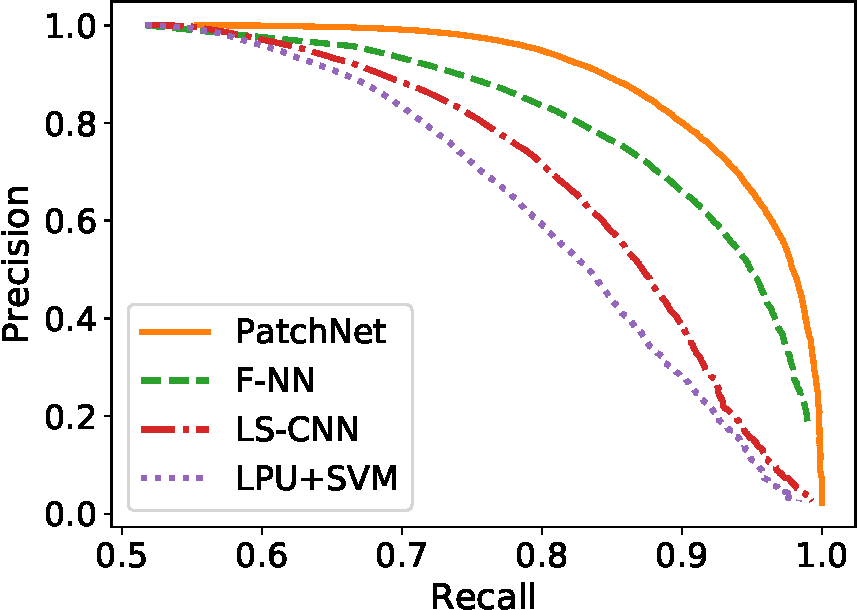
\includegraphics[scale=0.375]{figures/prc_recall_curve_ver1.pdf}
	\caption{Precision-recall curve: PatchNet vs. LPU+SVM, LS-CNN, and F-NN.}
	\label{fig:prc_rc_curve}
    \vspace{-0.4cm}
\end{figure}

% \begin{figure}
% % \centering
% % 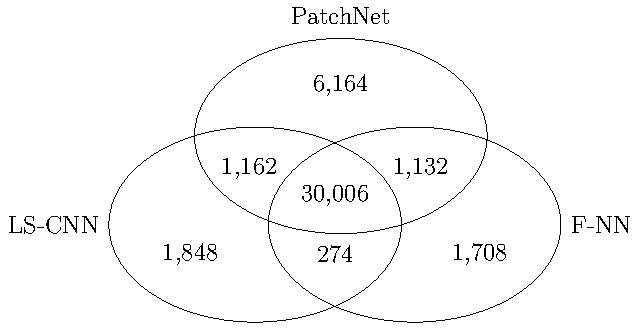
\includegraphics[scale=0.45]{figures/ven_diagram_ver1.pdf}
% % 	\caption{A Venn diagram showing overlapping of stable patches in three different algorithms, i.e., PatchNet, F-NN, and LS-CNN.}
% % 	\label{fig:venn_diagram}
% %     \vspace{-0.4cm}
% \def\first{(-.2,0) ellipse (6em and 3em)}
% \def\second{(1,0) ellipse (6em and 3em)}
% \def\third{(0.4,0.5) ellipse (6em and 3em)}
% \centerline{\begin{tikzpicture} \scriptsize
%     \draw \first node [below] (An) {};
%     \draw \second node [below] (Bn) {};
%     \draw \third node [above] (Cn) {};
% %
%     % first coordinate control x axis, second controls y axis
%     \node at (-1.1,-.2) (A) {1,848};
%     \node at (1.9,-.2) (B) {1,708};
%     \node at (.4,.95) (C) {6,164};
% %
%     \node at (.4,.2) {30,006};
% %
%     \node at (.4,-.4) {274}; % LS-CNN and F-NN
%     \node at (-0.65,.4) {1,162}; % LS-CNN and PatchNet
%     \node at (1.45,.4) {1,132}; % F-CNN and PatchNet
% %
%     \node[anchor=east] at (-1.7,0) {LS-CNN};
%     \node[anchor=west] at (2.5,0) (B) {F-NN};
%     \node[anchor=south] at (0.4,1.3) (C) {PatchNet};
% %
%   \end{tikzpicture}}
% 	\caption{A Venn diagram showing overlapping of stable patches in three different algorithms, i.e., PatchNet, F-NN, and LS-CNN.}
% 	\label{fig:venn_diagram}
% \end{figure}

\begin{figure}
\def\firsta{(-.2,0) ellipse (6em and 3em)}
\def\seconda{(1,0) ellipse (6em and 3em)}
\def\thirda{(0.4,0.5) ellipse (6em and 3em)}
\centerline{\begin{tikzpicture} \scriptsize
    \draw \firsta node [below] (An) {};
    \draw \seconda node [below] (Bn) {};
    \draw \thirda node [above] (Cn) {};
%
    % first coordinate control x axis, second controls y axis
    \node at (-1.1,-.2) (A) {1,109};
    \node at (1.9,-.2) (B) {1,905};
    \node at (.4,.95) (C) {6,785};
%
    \node at (.4,.2) {20,003};
%
    \node at (.4,-.4) {217}; % LS-CNN and F-NN
    \node at (-0.65,.4) {511}; % LS-CNN and PatchNet
    \node at (1.45,.4) {11,165}; % F-CNN and PatchNet
%
    \node[anchor=east] at (-1.7,0) {Keyword};
    \node[anchor=west] at (2.5,0) (B) {LS-CNN};
    \node[anchor=east] at (-.8,1.1) (C) {PatchNet};
%
  \end{tikzpicture}}

\vspace{\baselineskip}

\def\first{(-.2,0) ellipse (6em and 3em)}
\def\second{(1,0) ellipse (6em and 3em)}
\def\third{(0.4,0.5) ellipse (6em and 3em)}
\centerline{\begin{tikzpicture} \scriptsize
    \draw \first node [below] (An) {};
    \draw \second node [below] (Bn) {};
    \draw \third node [above] (Cn) {};
%
    % first coordinate control x axis, second controls y axis
    \node at (-1.1,-.2) (A) {1,296};
    \node at (1.9,-.2) (B) {1,784};
    \node at (.4,.95) (C) {6,572};
%
    \node at (.4,.2) {27,516};
%
    \node at (.4,-.4) {198}; % LS-CNN and F-NN
    \node at (-0.65,.4) {754}; % LS-CNN and PatchNet
    \node at (1.45,.4) {3,622}; % F-CNN and PatchNet
%
    \node[anchor=east] at (-1.7,0) {LPU-SVM};
    \node[anchor=west] at (2.5,0) (B) {F-NN};
    \node[anchor=east] at (-.8,1.1) (C) {PatchNet};
%
  \end{tikzpicture}}
	\caption{Venn diagrams showing the number of stable
          patches identified by PatchNet and the various baselines}
	\label{fig:venn_diagram}
\end{figure}

\vspace{0.1cm}\noindent{\bf RQ3: Does PatchNet benefit from considering
  both the commit message and the code changes, and do function names help
  identify stable patches?}  To answer this RQ, we conduct an ablation
test~\cite{korbar2017deep, liu2017deep}
% \jg{recheck refs} 
by ignoring the
commit message, the code changes, or the function names in the code changes
in a given patch one-at-a-time and evaluating the performance. We create
three variants of PatchNet: PatchNet-C, PatchNet-M, and
PatchNet-NN. PatchNet-C uses only code change information while PatchNet-M
uses only commit message information. PatchNet-NN uses both code change and
commit message information, but ignores the function names in the code
changes. We again use the five copies of the dataset described in RQ1 and
compute the various evaluation metrics.

Table~\ref{tab:components} shows that the performance of PatchNet degrades
if we ignore any one of the considered types of information. Accuracy,
precision, recall, F1, and AUC drop by 19.39\%, 15.41\%, 21.26\%, 18.34\%,
and 16.06\% respectively if we ignore commit messages. They drop by 16.96\%,
14.62\%, 16.58\%, 14.76\%, and 14.21\% respectively if we ignore code
changes.  And they drop by 11.08\%, 12.62\%, 16.43\%, 13.86\%, and 11.98\%
respectively if we ignore function names.  Thus, each kind of information
contributes to PatchNet's performance.  Additionally, the drops are
greatest if we ignore commit messages, indicating that they are slightly
more important than the other two to PatchNet's performance.

\begin{table}[t!]
  \centering
  \caption{Contribution of commit messages and code changes to PatchNet's performance}
    \begin{tabular}{|l|c|c|c|c|c|}
    \hline
          & \textbf{Accuracy} & \textbf{Precision} & \textbf{Recall} & \textbf{F1}    & \textbf{AUC} \\
    \hline
    \hline
    PatchNet-C & 0.722 & 0.727 & 0.748 & 0.736 & 0.741 \\
    \hline
    PatchNet-M & 0.737 & 0.732 & 0.778 & 0.759 & 0.753 \\
    \hline
    PatchNet-NN & 0.776 & 0.745 & 0.779 & 0.765 & 0.768 \\
    \hline
    PatchNet & \textbf{0.862} & \textbf{0.839} & \textbf{0.907} & \textbf{0.871} & \textbf{0.860} \\
    \hline
    \end{tabular}%
  \label{tab:components}%
\end{table}%

% % Table generated by Excel2LaTeX from sheet 'Sheet5'
% \begin{table}[t!]
%   \centering
%   \caption{CODE}
%     \begin{tabular}{|l|c|c|c|c|c|}
%     \hline
%           & Accuracy & Precision & Recall & F1    & AUC \\
%     \hline
%     \hline
%     BugFix & -     & -     & -     & -     & - \\
%     \hline
%     LPU-SVM & 0.649 & 0.817 & 0.571 & 0.672 & 0.676 \\
%     \hline
%     LS-CNN & 0.726 & 0.829 & 0.69  & 0.753 & 0.754 \\
%     \hline
%     PatchNet & \textbf{0.769} & \textbf{0.859} & \textbf{0.697} & \textbf{0.77} & \textbf{0.752} \\
%     \hline
%     \end{tabular}%
%   \label{tab:code}%
% \end{table}%

% \begin{table}[t!]
%   \centering
%   \caption{CODE}
%     \begin{tabular}{|l|c|c|c|c|c|}
%     \hline
%           & \textbf{Accuracy} & \textbf{Precision } & \textbf{Recall } & \textbf{F1} & \textbf{AUC} \\
%     \hline
%     \hline
%     BugFix & -     & -     & -     & -     & - \\
%     \hline
%     LPU+SVM & -     & -     & -     & -     & - \\
%     \hline
%     DTree & 0.561 & 0.574 & 0.583 & 0.578 & 0.56 \\
%     \hline
%     LSTM  & 0.584 & 0.568 & 0.821 & 0.671 & 0.576 \\
%     \hline
%     Bi-LSTM & 0.577 & 0.570  & 0.741 & 0.644 & 0.571 \\
%     \hline
%     CNN   & 0.579 & 0.570  & 0.757 & 0.650  & 0.573 \\
%     \hline
%     LSTM-CNN & 0.583 & 0.574 & 0.748 & 0.649 & 0.577 \\
%     \hline
%     PatchNet & \textbf{0.654} & \textbf{0.675} & \textbf{0.719} & \textbf{0.696} & \textbf{0.655} \\
%     \hline
%     \end{tabular}%
%   \label{tab:code}%
% \end{table}%

% \begin{table}[t!]
%   \centering
%   \caption{Add caption}
%     \begin{tabular}{|l|c|c|c|c|c|}
%     \hline
%           & \textbf{Accuracy} & \textbf{Precision } & \textbf{Recall } & \textbf{F1} & \textbf{AUC} \\
%     \hline
%     \hline
%     BugFix & 0.626 & 0.683 & 0.515 & 0.587 & 0.63 \\
%     \hline
%     LPU+SVM & -     & -     & -     & -     & - \\
%     \hline
%     DTree & 0.64  & 0.653 & 0.649 & 0.651 & 0.64 \\
%     \hline
%     LSTM  & 0.672 & 0.68  & 0.689 & 0.684 & 0.671 \\
%     \hline
%     Bi-LSTM & 0.668 & 0.698 & 0.629 & 0.661 & 0.669 \\
%     \hline
%     CNN   & 0.678 & 0.686 & 0.695 & 0.691 & 0.678 \\
%     \hline
%     LSTM-CNN & 0.668 & 0.698 & 0.629 & 0.661 & 0.669 \\
%     \hline
%     PatchNet & \textbf{0.680} & \textbf{0.677} & \textbf{0.728} & \textbf{0.701} & \textbf{0.678} \\
%     \hline
%     \end{tabular}%
%   \label{tab:msg}%
% \end{table}%

% \begin{table}[t!]
%   \centering
%   \caption{MSG}
%     \begin{tabular}{|l|c|c|c|c|c|}
%     \hline
%           & Accuracy & Precision & Recall & F1    & AUC \\
%     \hline
%     \hline
%     BugFix & 0.690  & 0.925 & 0.555 & 0.693 & 0.738 \\
%     \hline
%     LPU-SVM & 0.718 & 0.838 & 0.684 & 0.753 & 0.730 \\
%     \hline
%     LS-CNN & 0.762 & 0.896 & 0.688 & 0.778 & 0.780 \\
%     \hline
%     PatchNet & \textbf{0.775} & \textbf{0.902} & \textbf{0.710} & \textbf{0.794} & \textbf{0.799} \\
%     \hline
%     \end{tabular}%
%   \label{tab:msg}%
% \end{table}%

% \begin{table}[t!]
%   \centering
%   \caption{Add caption}
%     \begin{tabular}{|l|c|c|c|c|c|}
%     \hline
%           & Accuracy & Precision & Recall & F1    & AUC \\
%     \hline
%     \hline
%     PatchNet-C & 0.769 & 0.859 & 0.697 & 0.77  & 0.752 \\
%     \hline
%     PatchNet-M & 0.775 & 0.902 & 0.71  & 0.794 & 0.799 \\
%     \hline
%     PatchNet & \textbf{0.836} & \textbf{0.962} & \textbf{0.77}  & \textbf{0.856} & \textbf{0.859} \\
%     \hline
%     \end{tabular}%
%   \label{tab:addlabel}%
% \end{table}%

 


%\section{Case Study}
\label{sec:case_study}
In this section, we present a detailed analysis of the results obtains in Setion~\ref{sec:exp}. We show examples to understand the scenarios in which the scenarios in which PatchNet would perform well or poorly in Section~\ref{sec:good_case} and~\ref{sec:fail_case}. 

\subsection{Successful Case}
\label{sec:good_case}

\begin{figure}[t!]
\begin{lstlisting}[language=diff]
commit 	82981930125abfd39d7c8378a9cfdf5e1be2002b
Author: Eric Dumazet <...>
Date:   Thu Apr 10 20:07:59 2012 +0000

    net: cleanups in sock_setsockopt()
    
    Use min_t()/max_t() macros, reformat two comments, ... 
    
    Signed-off-by: Eric Dumazet <...>
    Signed-off-by: David S. Miller <...>


diff --git a/net/core/sock.c b/net/core/sock.c
index 0431aaf7473a..10605d2ec860 100644
--- a/net/core/sock.c
+++ b/net/core/sock.c
@@ -577,23 +577,15 @@ int sock_setsockopt(...
...
-	if (val > sysctl_wmem_max)
-   		val = sysctl_wmem_max;
+	val = min_t(u32, val, sysctl_wmem_max);   
-	if ((val * 2) < SOCK_MIN_SNDBUF)
-		sk->sk_sndbuf = SOCK_MIN_SNDBUF;
-	else
-		sk->sk_sndbuf = val * 2;
+	sk->sk_sndbuf = max_t(u32, val * 2, SOCK_MIN_SNDBUF);
@@ -577,23 +577,15 @@ int sock_setsockopt(...
-	if (val > sysctl_rmem_max)
-		val = sysctl_rmem_max;
+	val = min_t(u32, val, sysctl_rmem_max);
@@ -629,10 +620,7 @@ set_rcvbuf:
...
\end{lstlisting}\vspace{-0.4cm}
\caption{A true positive for PatchNet that is not detected by the other
  baselines}
\label{fig:good_case}\vspace{-0.4cm}
\end{figure}
\jg{Julia: can you please take a look at this example to see whether it's a good example?}

Figure~\ref{fig:good_case} shows an example of stable patch~\footnote{https://goo.gl/Yfi4TZ} that PatchNet is able to classify as a stable patch while the other baselines classify it as a non-stable patch. We take a look at a textual commit message of this patch, we see that there are no keywords (i.e., ``bug'', `'fix'', etc.) which help to recognize whether the example is the stable and non-stable patch. 

On the other hand, the code changes may contain sufficient information that may help maintainers to label it as the stable patch. The other baselines (i.e., LPU+SVM, F-NN) mainly constructed code features based on the code changes information, i.e., number of loops in added or removed codes, number of lines in added or removed codes, etc. However, they don't capture the sequential nature of the source code inside the code changes. LS-CNN fails to understand the code changes structure, i.e., hunks, added code, and removed code. PatchNet learns the sequential nature of source code inside the code changes and takes into account the code changes structure, hence it is able to classify the example as the stable patch.  

\subsection{Unsuccessful Case}
\label{sec:fail_case}

\begin{figure}[t!]
\begin{lstlisting}[language=diff]
commit 	fad54440438a7c231a6ae347738423cbabc936d9
Author: Julian Anastasov <...>
Date:   Fri Aug 05 00:36:28 2011 +0000

    netfilter: avoid double free in nf_reinject
    NF_STOLEN means skb was already freed
    
    Signed-off-by: Julian Anastasov <...>
    Signed-off-by: David S. Miller <...>

diff --git a/net/netfilter/nf_queue.c b/net/netfilter/nf_queue.c
index 5b466cd1272f..84d0fd47636a 100644
--- a/net/netfilter/nf_queue.c
+++ b/net/netfilter/nf_queue.c
@@ -314,0 +315 @@ void nf_reinject(...)
+	break;
\end{lstlisting}\vspace{-0.4cm}
\caption{A false negative for PatchNet that is successfully detected as
  stable by F-NN}
\label{fig:bad_case}\vspace{-0.4cm}
\end{figure}

Figure~\ref{fig:bad_case} presents an example of the patch which PatchNet fails to label as a stable patch while F-NN is able to classify it as the stable patch. According to the figure, the patch does not contain much information in both commit message as well as commit code, hence PatchNet fails to classify it as the stable patch. We note that all baselines also fail to label this patch as well except F-NN. In our opinion, F-NN uses author names as features hence it may be able to correctly label this patch. 

\section{Threats to Validity}
\label{sec:threat}

\noindent {\em Internal Validity}: Threats to internal validity relate to
errors in our experiments and experimenter bias. We have double checked our
code and data, but there may still be errors that we are not aware of. In
the baseline approach by Tian et al.~\cite{tian2012identifying}, commits
were labeled by an author with expertise in Linux kernel code, which may
introduce author bias. In this work, none of the authors label the commits.

\vspace{0.1cm}\noindent {\em External Validity}: Threats to external
validity relate to the generalizability of our approach. We have evaluated
our approach on more than 80,000 patches. We believe this is a good number
of patches; still, the results may differ if we consider other sets of
Linux kernel patches. Similar to the evaluation of Tian et
al.~\cite{tian2012identifying}, we only investigated Linux kernel patches,
although PatchNet can be applied to patches of other systems, if
labels are available. In the
future, we would like to consider more projects.
Still, we note that the Linux kernel represents one of the largest open
source projects, with over 16 million lines of C code, and that different
kernel subsystems have very different purposes, resulting in a wide variety
of code.

\vspace{0.1cm}\noindent {\em Construct Validity}: Threats to construct validity relate to the suitability of our evaluation metrics. We use standard metrics commonly used to evaluate classifier performance. Thus, we believe there is little threat to construct validity.





\section{Related Work}
\label{sec:related_work}

Researchers have applied deep learning techniques to solve software
engineering problems, including code clone
detection~\cite{white2016deep,li2017cclearner,bui2018hierarchical}, software traceability link
recovery~\cite{guo2017semantically}, bug
localization~\cite{huo2016learning, lam2017bug}, defect
detection~\cite{yang2015deep, wang2016automatically}, automated program
repair~\cite{gupta2017deepfix}, and API
learning~\cite{gu2016deep}. However, we did not find any work that applied
deep learning techniques to learn semantic representations of patches for
similar tasks such as stable patch identification, patch classification, etc. Here, we briefly describe the most closely related work besides the baseline approaches described in Section~\ref{sec:baselines}.


%\vspace{0.1cm} \noindent {\em Sequence-to-sequence learning.} Gu et al. adopted a neural language model named a Recursive Neural Network (RNN)~\cite{hagan1996neural, mikolov2010recurrent} encoder-decoder to generate API usage sequences, i.e., a sequence of method names, for a given natural language query~\cite{gu2016deep}. Gupta et al. proposed DeepFix to automatically fix syntax errors in C code~\cite{gupta2017deepfix}. DeepFix leverages a multi-layered sequence-to-sequence neural network with attention~\cite{mnih2014recurrent}, to process the input code and a decoder RNN with attention that generates the output fixed code. The above studies focus on learning sequence-to-sequence mappings and thus consider a different task than the one considered in our work.

%\vspace{0.1cm} \noindent {\em Learning code representation.}
CCLearner~\cite{li2017cclearner} learns a deep neural network classifier
from clone pairs and non clone pairs to detect clones.  To represent code,
it extracts features based on different categories (reserved words,
operators, etc.) of tokens in source code. White et al. presented another
deep learning based clone detector~\cite{white2016deep}. Their tool first
uses RNN to map program tokens to continuous-valued vectors, and then uses
RNN to combine the vectors with extracted syntactic features to train a
classifier. Wang et al. used a Deep Belief Network
(DBN)~\cite{hinton2009deep} to predict defective
code~\cite{wang2016automatically}. The DBN learns a semantic representation
(in the form of a continuous-valued vector) of each source code file from
token vectors extracted from programs' ASTs. Lam et al. combined deep
learning with information
retrieval to localize
buggy files based on bug reports~\cite{lam2017bug}. Bui and Jiang
proposed a deep learning based approach to automatically learn
cross-language representations for various kinds of structural code
elements (i.e., expressions, statements, and methods) for program
translation~\cite{bui2018hierarchical}. Different from the above
studies, we design a novel deep learning architecture that focuses on code
changes, taking into account their hierarchical and structural properties.

%Different from the above studies, we design a novel deep learning solution that: (1) learns representations of both text (in our case, commit logs) and code, and (2) considers code changes (i.e., diffs) rather than a source code file. 
%and (3) considers the hierarchical and sequential structure of code changes.


%\vspace{0.1cm} \noindent {\em Learning of both code and text representations.} Huo and Li proposed a model, LS-CNN, for classifying if a source code file is related to a bug report (i.e., the source code file needs to be fixed to resolve the bug report)~\cite{huo2017enhancing}. LS-CNN is the first code representation learning method that combines CNN and LSTM (a specific type of RNN) to extract semantic representations from \jl{from or of?} both code (in their case: a source code file) and text (in their case: a bug report). Similar to LS-CNN, PatchNet also learns semantic representations of \jl{from or of?} both code and text. However, different from LS-CNN, PatchNet includes a new representation learning architecture for commit code comprising the representations of removed code and added code of an affected file in a given patch. The representation of removed code and added code is able to capture the sequential nature of the source code inside a code change and it is learned following a CNN-3D architecture~\cite{ji20133d}, instead of LSTM. Our results in Section~\ref{sec:exp} show that PatchNet can achieve an 11.24\% improvement in terms of F1 over the LS-CNN model.

%\jl{The following seemed out of place in Section 3:}
%\jg{I'll ask Tian Yuan to take a look at this part.}
%Tian et al.~\cite{tian2012identifying} manually extracted code change features, i.e., number of files, number of hunks, etc., from a set of diff code changes, but that work does not break up the code changes by a file. Features extracted from code changes for each file may provide more information about the overall code changes by a given patch.

\vspace{-0.1cm}
\section{Conclusion}
\label{sec:conclusion}

In this paper, we propose PatchNet, a hierarchical deep learning-based model for identifying stable patches in the Linux kernel. For each patch, our model constructs embedding vectors from the commit message and the set of code changes. The embedding vectors are concatenated and then used to compute a prediction score for the patch. Different from existing deep learning techniques working on the source code~\cite{white2016deep, wang2016automatically, huo2017enhancing, li2017cclearner, guo2017semantically, lam2017bug, gu2016deep}, our hierarchical deep learning-based architecture takes into account the structure of code changes (i.e., files, hunks, lines) and the sequential nature of source code (by considering each line of code as a sequence of words) to predict stable patches in Linux kernel. 

% PatchNet learns a representation of code changes by constructing embedding vectors of removed and added code of an affected file in the given patch. We concatenate these embedding vectors to construct an embedding vector of the affected file. The embedding vector is subsequently used to extract the representation of the code changes. \jg{rephrase this sentence}

We have extensively evaluated PatchNet on a new dataset containing 82,403 recent Linux kernel patches. The results show that PatchNet outperforms 
% the best-performing baseline (F-NN) by 6.55\%, 7.8\%, and 6.3\% 
% in terms of accuracy, F1, and AUC, respectively. We also notice that 
four different baselines including two also based on deep-learning. In particular, for a wide range of values in the precision-recall curve, PatchNet obtains the highest recall for a given precision; as well as the highest precision for a given recall. For example, PatchNet achieves a 14.9\% higher recall (0.786) at a high precision level (0.95) and a 41.2\% higher precision (0.603) at a high recall level (0.95) compared to the best-performing baseline.

% Our representation of code changes includes names of non-local functions
% that are used at least 5 times, but no other variable names.  A possible
% future direction would be to investigate whether more kinds of names could
% be retained, to improve the learned result without over diversifying the
% dataset.  Another issue in identifying stable-relevant patches is to identify
% which earlier stable versions the patch should be applied to.  We will
% investigate whether machine learning can be used to help with this issue.
% \jl{David had comments for this paragraph}

In future work, we want to investigate ways to improve
our approach further, {\em e.g.}, by incorporating additional data such as
more kinds of names and type information.  Another issue would be to
identify the stable versions to which a patch should be applied. We plan to
investigate whether machine learning can help with this issue.  It would
also be interesting apply our approach that learns patch (diff) embeddings
to other related problems, {\em e.g.} identification of valid/invalid patches in
automated program repair~\cite{xiong2018identifying}, assignment of patches
to developers for code review~\cite{thongtanunam2015should,
zanjani2016automatically}, etc.

%\appendix
\section{Some examples}

The following illustrate some cases of stable patches that are recognized
only by PatchNet.

\begin{lstlisting}[language=diff]
commit 5567e989198b5a8d78f9b5868e48fc9f4726bdd5
Author: Madalin Bucur <...>
Date:   Mon Jun 19 18:04:16 2017 +0300

    fsl/fman: propagate dma_ops
    
    Make sure dma_ops are set, to be later used by the Ethernet driver.
    
    Signed-off-by: Madalin Bucur <...>
    Signed-off-by: David S. Miller <...>

diff --git a/drivers/net/ethernet/freescale/fman/mac.c b/...
index 0b31f8502ada..6e67d22fd0d5 100644
--- a/drivers/net/ethernet/freescale/fman/mac.c
+++ b/drivers/net/ethernet/freescale/fman/mac.c
@@ -625,0 +626,2 @@
+       set_dma_ops(&pdev->dev, get_dma_ops(priv->dev));
+

commit 2e31b4cb895ae78db31dffb860cd255d86c6561c
Author: Trond Myklebust <...>
Date:   Tue Jun 27 17:40:50 2017 -0400

    NFSv4.1: nfs4_callback_free_slot() cannot call nfs4_slot_tbl_drain_complete()
    
    The current code works only for the case where we have exactly one slot,
    which is no longer true.
    nfs4_free_slot() will automatically declare the callback channel to be
    drained when all slots have been returned.
    
    Signed-off-by: Trond Myklebust <...>

diff --git a/fs/nfs/callback_xdr.c b/fs/nfs/callback_xdr.c
index c14758e08d73..390ac9c39c59 100644
--- a/fs/nfs/callback_xdr.c
+++ b/fs/nfs/callback_xdr.c
@@ -756 +755,0 @@
-       nfs4_slot_tbl_drain_complete(tbl);
\end{lstlisting}

The following illustrate some cases of stable patches that are not recognized
by PatchNet, but are recognized by at least one of the baselines.

\begin{lstlisting}[language=diff]
commit 03f219041fdbeb31cecff41bb1cb4e1018f9cf75
Author: Luis Henriques <lhenriques@suse.com>
Date:   Wed May 17 12:21:07 2017 +0100

    ceph: check i_nlink while converting a file handle to dentry
    
    Converting a file handle to a dentry can be done call after the inode
    unlink.  This means that __fh_to_dentry() requires an extra check to
    verify the number of links is not 0.
    
    The issue can be easily reproduced using xfstest generic/426, which does
    something like:
    
        name_to_handle_at(&fh)
        echo 3 > /proc/sys/vm/drop_caches
        unlink()
        open_by_handle_at(&fh)
    
    The call to open_by_handle_at() should fail, as the file doesn't exist
    anymore.
    
    Link: http://tracker.ceph.com/issues/19958
    Signed-off-by: Luis Henriques <lhenriques@suse.com>
    Reviewed-by: "Yan, Zheng" <zyan@redhat.com>
    Signed-off-by: Ilya Dryomov <idryomov@gmail.com>

diff --git a/fs/ceph/export.c b/fs/ceph/export.c
index e8f11fa565c5..7df550c13d7f 100644
--- a/fs/ceph/export.c
+++ b/fs/ceph/export.c
@@ -93,0 +94,4 @@
+               if (inode->i_nlink == 0) {
+                       iput(inode);
+                       return ERR_PTR(-ESTALE);
+               }

commit 56199016e8672feb7b903eda003a863d5bf2b8c4
Author: Yan, Zheng <zyan@redhat.com>
Date:   Thu Jun 1 16:44:53 2017 +0800

    ceph: use current_kernel_time() to get request time stamp
    
    ceph uses ktime_get_real_ts() to get request time stamp. In most
    other cases, current_kernel_time() is used to get time stamp for
    filesystem operations (called by current_time()).
    
    There is granularity difference between ktime_get_real_ts() and
    current_kernel_time(). The later one can be up to one jiffy behind
    the former one. This can causes inode's ctime to go back.
    
    Signed-off-by: "Yan, Zheng" <zyan@redhat.com>
    Signed-off-by: Ilya Dryomov <idryomov@gmail.com>

diff --git a/fs/ceph/mds_client.c b/fs/ceph/mds_client.c
index f38e56fa9712..0c05df44cc6c 100644
--- a/fs/ceph/mds_client.c
+++ b/fs/ceph/mds_client.c
@@ -1690 +1689,0 @@
-       struct timespec ts;
@@ -1709,2 +1708,2 @@
-       ktime_get_real_ts(&ts);
-       req->r_stamp = timespec_trunc(ts, mdsc->fsc->sb->s_time_gran);
+       req->r_stamp = timespec_trunc(current_kernel_time(),
+                                     mdsc->fsc->sb->s_time_gran);
\end{lstlisting}

\appendix
\section{Some examples}

To illustrate the effect of our approach, we provide a few mainline Linux
kernel commit ids\footnotemark[4] from our results.  Examples of true
positives not found by the other baselines ({\em cf.}
Figure \ref{fig:venn_diagram}) include 5567e989198b and 2e31b4cb895a.
Examples of false negatives found by at least one other baseline include
03f219041fdb and 56199016e867.  Most of PatchNet's top 100 false positives
appear to the authors to be stable-relevant patches that have been
overlooked by kernel maintainers.  Examples include e2bd416f6246 and
acf2dc2266b9.


\balance
\bibliographystyle{IEEEtran}
\bibliography{references} 
\end{document}
